\documentclass[
    table,
    12pt,
    oneside,
    a4paper,
    italian
]{book}

\PassOptionsToPackage{dvipsnames}{xcolor} % colori PDF/A

\usepackage{colorprofiles}
% PDF/A
% validate in https://www.pdf-online.com/osa/validate.aspx
\usepackage[a-1a,mathxmp]{pdfx}[2018/12/22]
\usepackage[T1]{fontenc}
\usepackage[utf8]{inputenc}
\usepackage[italian]{babel}
\usepackage{bookmark}
\usepackage{caption}
\usepackage{comment}
\usepackage{chngpage, calc} % centra il frontespizio
\usepackage{emptypage} % pagine vuote senza testatina e piede di pagina
\usepackage{epigraph} % per epigrafi
\usepackage{indentfirst} % rientra il primo paragrafo di ogni sezione
\usepackage{graphicx} % immagini
\usepackage[pdfa]{hyperref} % collegamenti ipertestuali
\usepackage{mparhack,relsize}  % finezze tipografiche
\usepackage{nameref} % visualizza nome dei riferimenti
\usepackage[font=small]{quoting} % citazioni
\usepackage{subfig} % sottofigure, sottotabelle
\usepackage[italian]{varioref} % riferimenti completi della pagina
\usepackage{longtable} % tabelle su più pagine
\usepackage[toc, acronym, automake]{glossaries}
\usepackage[backend=biber, style=verbose-ibid, hyperref, backref]{biblatex}
\usepackage{lmodern}
\usepackage[top=2.75cm, bottom=2.75cm, right=3cm, left=3.75cm]{geometry} % 1in+17pt+0.6cm
\usepackage{fancyhdr}
\usepackage{lipsum}
\usepackage{setspace}
\usepackage{titlesec}
\usepackage[cachedir=minted-caches]{minted} % https://it.overleaf.com/learn/latex/Code_Highlighting_with_minted
\usepackage{xcolor}
\usepackage{csquotes} % gestisce automaticamente i caratteri (")
\usepackage{etoolbox}
\usepackage[bottom]{footmisc}
\usepackage{zref-totpages}
% Load variables
\newcommand{\myUni}{Università degli Studi di Padova}
\newcommand{\myDepartment}{Dipartimento di Matematica ``Tullio Levi-Civita''}
\newcommand{\myFaculty}{Corso di Laurea in Informatica}
\newcommand{\myTitle}{Un sistema Honeypot per l'analisi di attacchi informatici in ambiente controllato}
\newcommand{\myDegree}{Tesi di Laurea Triennale}
\newcommand{\profTitle}{Prof.}
\newcommand{\myProf}{Vardanega Tullio}
\newcommand{\graduateTitle}{Laureando}
\newcommand{\myName}{Marko Peric}
\newcommand{\myStudentID}{2011067}
\newcommand{\myAA}{2024-2025}
\newcommand{\myLocation}{Padova}
\newcommand{\myTime}{Agosto 2025}
% Acronyms
\newacronym{tsa}{TSA}{Termine solo acronimo}

% Glossary

\newglossaryentry{TermineSenzaAcronimo}{
    name={Nome del termine},
    sort=termine senza acronimo,
    description={Descrizione}
}
\PassOptionsToPackage{dvipsnames}{xcolor} % colori PDF/A

\usepackage{colorprofiles}
% PDF/A
% validate in https://www.pdf-online.com/osa/validate.aspx
\usepackage[a-1a,mathxmp]{pdfx}[2018/12/22]
\usepackage[T1]{fontenc}
\usepackage[utf8]{inputenc}
\usepackage[italian]{babel}
\usepackage{bookmark}
\usepackage{caption}
\usepackage{comment}
\usepackage{chngpage, calc} % centra il frontespizio
\usepackage{emptypage} % pagine vuote senza testatina e piede di pagina
\usepackage{epigraph} % per epigrafi
\usepackage{indentfirst} % rientra il primo paragrafo di ogni sezione
\usepackage{graphicx} % immagini
\usepackage[pdfa]{hyperref} % collegamenti ipertestuali
\usepackage{mparhack,relsize}  % finezze tipografiche
\usepackage{nameref} % visualizza nome dei riferimenti
\usepackage[font=small]{quoting} % citazioni
\usepackage{subfig} % sottofigure, sottotabelle
\usepackage[italian]{varioref} % riferimenti completi della pagina
\usepackage{longtable} % tabelle su più pagine
\usepackage[toc, acronym, automake]{glossaries}
\usepackage[backend=biber, style=verbose-ibid, hyperref, backref]{biblatex}
\usepackage{lmodern}
\usepackage[top=2.75cm, bottom=2.75cm, right=3cm, left=3.75cm]{geometry} % 1in+17pt+0.6cm
\usepackage{fancyhdr}
\usepackage{lipsum}
\usepackage{setspace}
\usepackage{titlesec}
\usepackage[cachedir=minted-caches]{minted} % https://it.overleaf.com/learn/latex/Code_Highlighting_with_minted
\usepackage{xcolor}
\usepackage{csquotes} % gestisce automaticamente i caratteri (")
\usepackage{etoolbox}
\usepackage[bottom]{footmisc}
\usepackage{zref-totpages}

% Define custom colors
\definecolor{hyperColor}{HTML}{0B3EE3}
\definecolor{tableGray}{HTML}{F5F5F7}
\definecolor{veryPeri}{HTML}{6667ab}

% Set line height
\linespread{1.5}

% Custom hyphenation rules
\hyphenation {
    data-base
    al-go-rithms
    soft-ware
}

% Images path
\graphicspath{{img/}}

% Force page color, as some editors set a grayish color as default
\pagecolor{white}

% Better spacing for footnotes
\setlength{\skip\footins}{5mm}
\setlength{\footnotesep}{5mm}

\setlength{\headheight}{14.5pt}
\addtolength{\topmargin}{-2.45pt}

% Add a subscript G to a glossary entry
\newcommand{\glox}{\textsubscript{\textbf{\textit{G}}}}

% Improvements the paragraph command
\titleformat{\paragraph}
{\normalfont\normalsize\bfseries}{\theparagraph}{1em}{}
\titlespacing*{\paragraph}
{0pt}{3.25ex plus 1ex minus .2ex}{1.5ex plus .2ex}

% Define use case environment
\newcounter{usecasecounter} % define a counter
\setcounter{usecasecounter}{0} % set the counter to some initial value
% Parameters
% #1: ID
% #2: Nome
\newenvironment{usecase}[2]{
    \renewcommand{\theusecasecounter}{\usecasename #1}  % this is where the display of the counter is overwritten/modified
    \refstepcounter{usecasecounter} % increment counter
    \vspace{2em}
    \par \noindent % start new paragraph
    {\normalsize \textbf{\usecasename #1: #2}} % display the title before the content of the environment is displayed
    \vspace{.5em}
}{
    \medskip
}
\newcommand{\usecasename}{UC}
\newcommand{\usecaseactors}[1]{\textbf{\\Attori Principali:} #1}
\newcommand{\usecasepre}[1]{\textbf{\\Precondizioni:} #1}
\newcommand{\usecasedesc}[1]{\textbf{\\Descrizione:} #1}
\newcommand{\usecasepost}[1]{\textbf{\\Postcondizioni:} #1}
\newcommand{\usecasealt}[1]{\textbf{\\Scenario Alternativo:} #1}

% Define risks environment
\newcounter{riskcounter} % define a counter
\setcounter{riskcounter}{0} % set the counter to some initial value
% Parameters
% #1: Title
\newenvironment{risk}[1]{
    \refstepcounter{riskcounter} % increment counter
    \par \noindent % start new paragraph
    \textbf{\arabic{riskcounter}. #1} % display the title before the content of the environment is displayed
}{
    \par\medskip
}
\newcommand{\riskname}{Rischio}
\newcommand{\riskdescription}[1]{\textbf{\\Descrizione:} #1.}
\newcommand{\risksolution}[1]{\textbf{\\Soluzione:} #1.}

% Apply fancy styling to pages
\pagestyle{fancy}
\fancyhf{}
\fancyhead[L]{\leftmark} % Places Chapter N. Chatper title on the top left
\fancyfoot[C]{\thepage} % Page number in the center of the footer

% Adds a blank page while increasing the page number
\newcommand\blankpage{ 
\clearpage
    \begingroup
    \null
    \thispagestyle{empty}
    \hypersetup{pageanchor=false}
    \clearpage
\endgroup
}

% Adds a blank page while increasing the page number
\newcommand\blankpagewithnumber{ 
  \clearpage
  \thispagestyle{plain} % Use plain page style to keep the page number
  \null
  \clearpage
}

% Increase page numbering
\newcommand\increasepagenumbering{
    \addtocounter{page}{+1}
}

% Make glossaries and bibliography
\makeglossaries
% Redefine the format for the glossary entries to be italic
\renewcommand*{\glstextformat}[1]{\textit{#1}\glox}
%\glsaddall

\bibliography{references/bibliography}
\defbibheading{bibliography} {
    \cleardoublepage
    \phantomsection
    \addcontentsline{toc}{chapter}{\bibname}
    \chapter*{\bibname\markboth{\bibname}{\bibname}}
}

% Code blocks handling w/ table of codes
\makeatletter
\ifdefined\NR@chapter
  \expandafter\@firstoftwo
\else
  \expandafter\@secondoftwo
\fi{\patchcmd\NR@chapter}{\patchcmd\@chapter}
  {\addtocontents{lot}{\protect\addvspace{10\p@}}}
  {\addtocontents{lot}{\protect\addvspace{10\p@}}%
   \addtocontents{lol}{\protect\addvspace{10\p@}}}
  {}{}
\makeatother

\renewcommand\listingscaption{Codice}
\renewcommand\listoflistingscaption{Elenco dei codici sorgenti}
\counterwithin*{listing}{chapter}
\renewcommand\thelisting{\thechapter.\arabic{listing}}

% Set up hyperlinks
\hypersetup{
    colorlinks=true,
    linktocpage=true,
    pdfstartpage=1,
    pdfstartview=,
    breaklinks=true,
    pdfpagemode=UseNone,
    pageanchor=true,
    pdfpagemode=UseOutlines,
    plainpages=false,
    bookmarksnumbered,
    bookmarksopen=true,
    bookmarksopenlevel=1,
    hypertexnames=true,
    pdfhighlight=/O,
    allcolors = hyperColor
}

% Set up captions
\captionsetup{
    tableposition=top,
    figureposition=bottom,
    font=small,
    format=hang,
    labelfont=bf
}

% When draft mode is on, the hyperlinks are removed. Useful when printing the document. To enable/disable, uncomment/comment the command
% \hypersetup{draft}

% prevents cleaning up the cache at the end of the run (needed to keep the unused caches, generated by other editions)
% \makeatletter
% \renewcommand*{\minted@cleancache}{}
% \makeatother

% Break lines in code blocks whe using inputminted
\setminted{breaklines}


\date{}

\hypersetup{pdfstartview=}
\begin{document}
    \frontmatter
    \begin{titlepage}
    \begin{center}
        \begin{Large}
            \textbf{\myUni}\\
        \end{Large}

        \vspace{5pt}

        \begin{large}
            \textsc{\myDepartment}\\
        \end{large}

        \vspace{5pt}

        \begin{large}
            \textsc{\myFaculty}\\
        \end{large}

        \vspace{25pt}
        
        \begin{figure}[htbp]
            \centering
            
\includegraphics[alt={Emblema dell'Università degli Studi di Padova}, height=6cm]{img/logo_unipd.jpeg}
        \end{figure}

        
        \begin{Large}
            \textbf{\myTitle}\\
        \end{Large}

        \vspace{5pt}

        \begin{large}
            \textit{\myDegree}\\
        \end{large}

        \vspace{50pt}
        
        \begin{normalsize}
            \begin{flushleft}
                \textit{Relatore}\\
                \profTitle\ \myProf
            \end{flushleft}

            \vspace{-48pt}
            
            \begin{flushright}
                \textit{\graduateTitle}\\
                \myName\\
                Matricola \myStudentID
            \end{flushright}
        \end{normalsize}

        \vspace*{\fill}
        
        \line(1, 0){338} \\
        \begin{normalsize}
            \textsc{Anno Accademico \myAA}
        \end{normalsize}
    \end{center}
\end{titlepage}

    \increasepagenumbering % increase the page numbrering by 1, in order to cout the frontispiece
    \clearpage
\phantomsection
\thispagestyle{empty}
\hfill
\vfill

{\small\noindent\textcopyright\ \myName, \myTime. Tutti i diritti riservati. \myDegree: ``\textit{\myTitle}'', \myUni, \myDepartment, \myFaculty.}
    \cleardoublepage
\phantomsection
\pdfbookmark{Ringraziamenti}{Ringraziamenti}

\begin{flushright}{
    \slshape
    ``Colui il quale ha inseguito e sconfitto i demoni Sem, che ora vagano per il mondo, domandandosi: «ma nü, chi sëm?»''} \\
    \medskip
    --- Il grande Pdor, figlio di Kmer, della tribù di Ishtar, della terra desolata dei Kfnir, uno degli ultimi sette saggi: Pfulur, Galér, Astaparigna, Sùsar, Param, Fusus e Tarìm.
\end{flushright}

\begingroup
\let\clearpage\relax
\let\cleardoublepage\relax
\let\cleardoublepage\relax

\chapter*{Ringraziamenti}

\noindent Desidero esprimere la mia gratitudine al professor \myProf, mio relatore, per l'aiuto e il sostegno che mi ha dato durante la stesura dell'elaborato.

\vspace{0.35cm}

\noindent Vorrei anche ringraziare, con affetto, i miei genitori per il loro sostegno, il grande aiuto e la loro presenza in ogni momento durante gli anni di studio.

\vspace{0.35cm}

\noindent Desidero poi ringraziare i miei amici per i bellissimi anni trascorsi insieme e le mille avventure vissute.

\vspace{0.75cm}

\noindent{\myLocation, \myTime}
\hfill \textit{\myName}

\endgroup

    \cleardoublepage
\phantomsection
\pdfbookmark{Compendio}{Compendio}
\begingroup
\let\clearpage\relax
\let\cleardoublepage\relax
\chapter*{Sommario}
Il presente elaborato descrive il lavoro svolto durante il periodo di \textit{stage}, della durata di circa
320 ore, dal laureando Marko Peric presso l'azienda Eurosystem S.p.A. dal 18/06/2024 al
13/08/2025.
L'elaborato illustra i processi, le metodologie e gli strumenti impiegati nella progettazione e nello sviluppo di un sistema \textit{honeypot} finalizzato al monitoraggio e alla rilevazione di attività malevole in rete. Il sistema si basa sull'installazione di servizi volutamente vulnerabili su un server Linux Debian, con lo scopo di attirare potenziali attaccanti e analizzarne i comportamenti. I \textit{log} generati dai servizi vengono successivamente raccolti, elaborati e trasferiti in InfluxDB per la loro conservazione, e resi disponibili tramite Grafana per consentire un'analisi e una visualizzazione efficace delle informazioni tramite \textit{dashboard}.
\section*{Struttura dell'elaborato}
In questa sezione viene presentata la struttura dell'elaborato, illustrando brevemente il contenuto di ciascun capitolo:
\begin{description}
    \item[{\hyperref[chap:]{Il primo capitolo}}] approfondisce il contesto aziendale in cui si è svolto lo \textit{stage}, fornendo una panoramica completa dell'azienda, dei suoi prodotti e servizi nel settore della \textit{cybersecurity}, degli strumenti tecnologici utilizzati e dell'organizzazione del \textit{team} di sicurezza informatica, analizzando inoltre l'approccio dell'azienda verso l'innovazione tecnologica;

    \item[{\hyperref[chap:]{Il secondo capitolo}}] identifica e analizza il problema alla base del progetto, definendo gli obiettivi specifici dello sviluppo del sistema \textit{honeypot}, i vincoli operativi e tecnici che hanno influenzato il lavoro, le prospettive di sviluppo futuro e le motivazioni personali che hanno guidato la scelta di questo percorso di \textit{stage};

    \item[{\hyperref[chap:]{Il terzo capitolo}}] documenta l'intero processo di sviluppo del sistema \textit{honeypot}, dall'analisi dei requisiti e dei casi d'uso alla progettazione dell'architettura, dalla fase di codifica alle attività di verifica e validazione, presentando il prodotto finale e valutando il grado di conformità rispetto ai requisiti iniziali;
    
    \item[{\hyperref[chap:]{Il quarto capitolo}}] presenta una valutazione retrospettiva dell'esperienza formativa, analizzando il raggiungimento degli obiettivi prefissati, le conoscenze tecniche acquisite nel campo della sicurezza informatica e le competenze professionali sviluppate durante il periodo di tirocinio presso l'azienda.
\end{description}
\section*{Criteri tipografici adottati}
Riguardo la stesura del testo, relativamente al elaborato sono state adottate le seguenti convenzioni tipografiche:
\begin{itemize}
	\item gli acronimi e le abbreviazioni sono raccolti in un'apposita sezione dedicata, denominata \hyperref[acronimi]{Elenco degli acronimi} e sono segnati con la seguente nomenclatura \gls{es};
    \item i termini ambigui o di uso non comune, invece, sono definiti all'interno del \hyperref[glossario]{Glossario} e sono segnati con la seguente nomenclatura \gls{esempio};
	\item i termini in lingua straniera o facenti parti del gergo tecnico sono evidenziati con il carattere \textit{corsivo}.
\end{itemize}
\endgroup
\vfill

    \cleardoublepage
\pdfbookmark{\contentsname}{tableofcontents}
\setcounter{secnumdepth}{5}
\setcounter{tocdepth}{5}     

\tableofcontents
\clearpage

\begingroup
    \let\clearpage\relax
    \let\cleardoublepage\relax
    \let\cleardoublepage\relax

    % Figures list
    \phantomsection
    \pdfbookmark{\listfigurename}{lof}
    \listoffigures
    \vspace*{8ex}

    % Tables list
    \phantomsection
    \pdfbookmark{\listtablename}{lot}
    \listoftables
\endgroup

\begingroup
    % Code list
    \phantomsection
    \pdfbookmark{\listoflistingscaption}{lol}
    \listoflistings
\endgroup

\cleardoublepage
    \blankpage % example of a blank page that also increases the page couter by 1

    \mainmatter
    \chapter{Contesto lavorativo}
Il primo capitolo fornisce una panoramica sull'azienda ospitante Eurosystem S.p.A., evidenziando le principali aree operative dell'azienda. 

\section{L'azienda}
Eurosystem S.p.A. è un'impresa informatica con sede principale a Villorba (TV), attiva nel settore della consulenza, dei prodotti e dei servizi di \gls{it}. L'azienda è presente sul territorio nazionale con otto sedi operative, distribuite principalmente nel Nord Italia. Tra queste, la sede di Tavagnacco (UD) riveste un ruolo centrale in quanto ospita il reparto dedicato alle attività di \textit{cybersecurity}, ambito in cui è stato svolto il tirocinio curricolare in modalità da remoto.  
Fondata con l'obiettivo di fornire soluzioni tecnologiche a supporto delle imprese, Eurosystem S.p.A. si rivolge prevalentemente al settore delle piccole e medie imprese, accompagnandole nei processi di digitalizzazione e nella gestione dei rischi informatici. L'azienda si caratterizza per un approccio che combina l'adozione di tecnologie consolidate con l'attenzione verso l'innovazione e la sicurezza delle infrastrutture digitali.  
Il reparto di \textit{cybersecurity} si distingue per la sua funzione trasversale, in quanto collabora sia con i clienti sia con gli altri reparti aziendali, integrando misure di protezione all'interno delle soluzioni tecnologiche fornite.  
L'attenzione di Eurosystem S.p.A. non è rivolta unicamente alla fornitura di servizi, ma anche al mantenimento e all'aggiornamento costante delle competenze del personale. La formazione continua rappresenta un elemento fondamentale: nei periodi di minore operatività, i \textit{team} dedicano tempo allo studio di nuove tematiche, all'analisi di strumenti emergenti e alla sperimentazione di metodologie utili a fronteggiare l'evoluzione costante delle minacce informatiche.  
\section{Prodotti e servizi offerti}  
Eurosystem S.p.A. offre una gamma di prodotti e servizi informatici pensati per garantire la protezione delle infrastrutture \textit{IT} aziendali. In particolare, il reparto di \textit{cybersecurity} si occupa di diverse attività fondamentali per la difesa e la continuità operativa delle organizzazioni.\\\\  
Un primo ambito riguarda \textbf{il monitoraggio e la risposta agli incidenti}. Il \gls{soc}\glsadd{soc_def} e i servizi di \gls{mdr}\glsadd{mdr_def} assicurano un controllo costante delle reti aziendali, con l'obiettivo di rilevare in tempo reale anomalie e potenziali minacce. Il \textit{team} esamina ogni incidente nel dettaglio mediante la raccolta e l'analisi dei \textit{log} e dei dati di rete, l'identificazione dei vettori di attacco e delle vulnerabilità sfruttate, l'isolamento delle minacce e il ripristino dei sistemi tramite soluzioni di \textit{backup} e \textit{disaster recovery}. A completamento del processo, il \textit{team} redige \textit{report} dettagliati contenenti analisi, azioni intraprese e raccomandazioni di miglioramento.\\\\  
Un secondo ambito è rappresentato dalle \textbf{verifiche di sicurezza}, svolte tramite attività di \textit{Cyber Analysis Assessment}. In questa fase rientrano il \textit{Vulnerability Management} e i \textit{Penetration Test}, strumenti fondamentali per individuare e valutare i punti deboli delle infrastrutture \textit{IT}. A ciò si affiancano i servizi di \textit{Phishing Assessment}, utili a misurare la resilienza degli utenti contro campagne fraudolente, e le attività di \textit{Threat Intelligence}, finalizzate a raccogliere e analizzare informazioni utili a prevenire attacchi futuri.  
\begin{figure}[H]
    \centering
    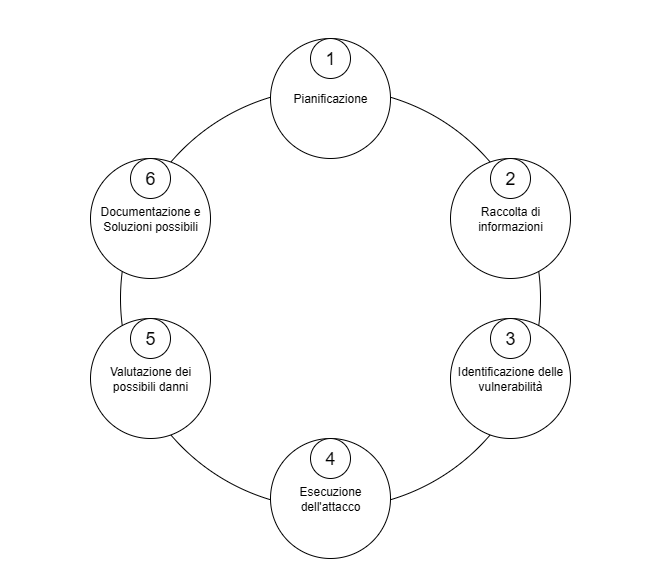
\includegraphics[alt={Schema Penetration Test}, width=0.95\columnwidth]{img/Pen_test.png}
    \caption{Schema di esempio di un processo di \textit{penetration testing}.}
    \label{fig:pen_test}    
\end{figure}  
\textbf{L'analisi delle reti} rappresenta un aspetto importante delle attività svolte. Questa comprende il monitoraggio del traffico di rete, il rilevamento di anomalie e la gestione degli eventi di sicurezza, con particolare attenzione alle reti industriali, al fine di contribuire alla continuità operativa dei processi produttivi.\\\\  
Un ruolo centrale è svolto anche dalla \textbf{gestione degli \textit{endpoint}}, ossia la protezione dei dispositivi aziendali, interni o remoti. Questa attività comprende il monitoraggio costante dello stato di sicurezza, l'applicazione degli aggiornamenti correttivi e delle politiche di protezione, il controllo delle identità e degli accessi, nonché il rilevamento e la risposta rapida alle minacce. Inoltre, sono previsti \textit{report} e \gls{audit} di conformità, volti a garantire trasparenza e allineamento con le normative.  
\begin{figure}[H]
    \centering
    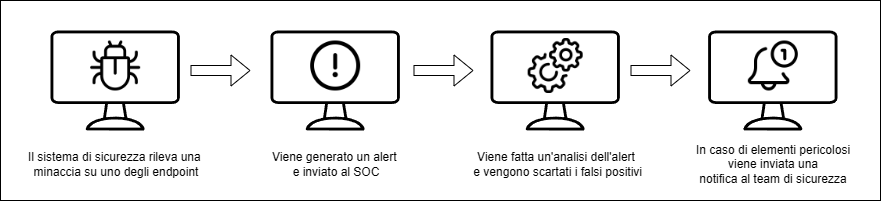
\includegraphics[alt={Schema Endpoint governance}, width=\columnwidth]{img/endpoint.png}
    \caption{Schema di esempio di un processo di gestione degli \textit{endpoint}.}
    \label{fig:endpoint_governance}    
\end{figure}  
Alla gestione degli \textit{endpoint} si affianca la \textbf{gestione dei dati}. Eurosystem S.p.A. supporta le aziende nella protezione, nell'organizzazione e nella conformità dei dati, in linea con i requisiti normativi, assicurando così un trattamento sicuro e affidabile delle informazioni.\\\\  
Un altro elemento di rilievo è la \textbf{gestione degli utenti e la sensibilizzazione}. L'azienda promuove attività formative mirate a diffondere buone pratiche di sicurezza informatica, con particolare attenzione agli accessi, ai privilegi e ai comportamenti corretti. In questo modo viene ridotto il rischio legato al fattore umano, spesso determinante nella riuscita di un attacco informatico.\\\\  
Infine, Eurosystem S.p.A. offre un \textbf{supporto tempestivo in caso di criticità}. In presenza di incidenti o sospette violazioni, i clienti ricevono un'assistenza diretta e immediata, con l'obiettivo di ridurre al minimo l'impatto sull'operatività aziendale.  
Grazie a questo insieme di attività, l'azienda è in grado di identificare proattivamente le vulnerabilità dei sistemi informativi, predisporre misure di protezione adeguate e garantire un aggiornamento costante delle competenze necessarie per affrontare l'evoluzione delle minacce informatiche.  

\section{Strumenti \textit{hardware}}
Nel caso in cui le attività lavorative vengano svolte da remoto, l'azienda mette a disposizione del lavoratore gli strumenti necessari per garantire il corretto svolgimento delle mansioni assegnate.
In particolare, l'azienda fornisce un computer portatile HP, configurato con l'account e la casella di posta elettronica aziendale, così da assicurare l'accesso immediato a tutte le risorse interne.
A supporto dell'utilizzo del dispositivo, è inoltre fornito un mouse.
\section{Strumenti \textit{software}}  
Le tecnologie e gli strumenti \textit{software} a supporto delle attività lavorative si articolano principalmente in due grandi categorie: strumenti organizzativi e strumenti produttivi.  
\subsection{Strumenti organizzativi}  
Per quanto riguarda gli strumenti organizzativi, l'azienda fa ampio uso di \textbf{\textit{Microsoft Teams}}, che rappresenta il principale canale di comunicazione interna. Questo strumento consente di coordinare le attività quotidiane, condividere documenti in modo rapido ed efficace e partecipare a riunioni o chiamate di lavoro quando necessario.\\\\
Un ruolo altrettanto centrale è ricoperto da \textbf{\textit{Microsoft Outlook}}, utilizzato non solo per la gestione della posta elettronica e dell'agenda, ma anche per la pianificazione di incontri e il mantenimento di un flusso di comunicazione costante, sia con i colleghi che con i clienti. \textit{Outlook} svolge inoltre una funzione cruciale nella ricezione di notifiche riguardanti incidenti di sicurezza provenienti da aziende esterne, garantendo così risposte tempestive in caso di necessità.\\\\
A completare questo insieme di strumenti organizzativi vi è \textbf{\textit{GitHub}}, adottato come piattaforma di controllo versione. Questo strumento consente la gestione strutturata del codice sorgente, il tracciamento delle modifiche e la collaborazione efficiente tra più sviluppatori.  
\subsection{Strumenti produttivi}  
Tra gli strumenti produttivi, un ruolo rilevante è svolto da \textbf{\textit{LaTeX}}, scelto per la redazione di documentazione tecnica e scientifica grazie alle sue elevate capacità di formattazione. La possibilità di gestire con precisione formule matematiche, grafici, bibliografie e glossari permette di ottenere documenti di elevata qualità tipografica. Il modello di separazione tra contenuto e presentazione rende inoltre il codice sorgente facilmente riutilizzabile e particolarmente adatto a contesti di collaborazione accademica e professionale.\\\\  
In parallelo, l'azienda fa un ampio utilizzo di \textbf{\textit{Python}}, linguaggio di programmazione versatile e diffuso, applicato soprattutto nel settore della \textit{cybersecurity}. Le sue potenzialità vengono sfruttate per automatizzare processi, analizzare file di \textit{log} e sviluppare strumenti di monitoraggio e rilevamento delle minacce, anche grazie alle numerose librerie specializzate che semplificano la creazione di script per il \textit{testing} della sicurezza, l'interazione con \gls{api}\glsadd{api_def} e la gestione di sistemi complessi.\\\\  
A supporto dello sviluppo i dipendenti adottano frequentemente \textbf{\textit{Visual Studio Code (VSCode)}}, un ambiente di programmazione leggero, modulare e altamente personalizzabile. Questo strumento è impiegato principalmente per la scrittura, il \textit{debugging} e la manutenzione del codice, offrendo un'ampia compatibilità con diversi linguaggi e la possibilità di integrare estensioni dedicate. Pur essendo l'\gls{ide}\gls{ide_def} più diffuso tra i dipendenti, la sua adozione non è vincolante: ciascun lavoratore può infatti optare per soluzioni alternative in base alle proprie esigenze e preferenze operative.\\\\  
Infine, un ulteriore strumento di grande rilevanza è \textbf{\textit{Docker}}, una tecnologia di virtualizzazione basata sui \gls{container}. Grazie a questo approccio, è possibile creare ambienti isolati, scalabili e facilmente replicabili. Docker, infatti, esegue le applicazioni includendo tutte le dipendenze necessarie. La leggerezza e portabilità della tecnologia ne favoriscono l'uso in fase di sviluppo, \textit{testing} e distribuzione, riducendo al minimo i problemi di compatibilità tra diversi sistemi.  

\section{Organizzazione del team}  

\subsection{\textit{Chief Information Security Officer} (CISO)}  
Il \textit{\gls{ciso}} è la figura responsabile della strategia di sicurezza informatica all'interno dell'azienda.
Supervisiona tutte le attività del reparto di \textit{cybersecurity} e ne garantisce la coerenza con gli obiettivi aziendali e con le normative vigenti.
Durante il periodo di tirocinio, questa figura ha ricoperto anche il ruolo di tutor aziendale, fornendo supporto e guida nelle varie attività.
Tra le sue principali responsabilità rientrano la definizione delle politiche e delle strategie di sicurezza, la supervisione delle attività operative del team, il coordinamento tra i diversi ruoli del reparto e la verifica della conformità agli standard di settore.
A ciò si aggiunge un impegno costante nel supporto e nella formazione interna, volto a diffondere buone pratiche di sicurezza informatica tra i dipendenti.  

\subsection{\textit{Penetration tester}}  
Il \textit{penetration tester} ha l'obiettivo di individuare le vulnerabilità presenti nei sistemi informatici attraverso l'esecuzione di attacchi simulati in un contesto controllato.
Il suo lavoro si articola in più fasi, che comprendono la pianificazione e l'esecuzione di \textit{penetration test}, la simulazione di scenari di attacco realistici e l'analisi delle debolezze riscontrate.
Al termine delle attività, il professionista redige report tecnici dettagliati nei quali vengono descritte le criticità emerse, corredati da proposte di contromisure e raccomandazioni operative, così da supportare l'azienda nell'adozione di strategie efficaci di mitigazione del rischio.  

\subsection{\textit{Security analyst}}  
Il \textit{security analyst} si occupa del monitoraggio costante dei sistemi informativi e della gestione operativa degli eventi di sicurezza, con l'obiettivo di rilevare tempestivamente potenziali incidenti e coordinare una risposta adeguata.
Le sue attività comprendono il controllo delle infrastrutture tramite strumenti avanzati di analisi, il rilevamento e la classificazione degli avvisi di sicurezza, nonché l'esame dei log e delle anomalie di rete.
In caso di incidenti, fornisce supporto operativo nelle attività di risposta e contribuisce alla definizione di procedure correttive.
Inoltre, elabora linee guida e buone pratiche da condividere con clienti e colleghi, contribuendo così a diffondere una maggiore consapevolezza in materia di sicurezza informatica.  

\section{Predisposizione all'innovazione}

L'ambito della \textit{cybersecurity} è caratterizzato da un'evoluzione continua: nuove vulnerabilità, strumenti di attacco e metodologie di compromissione emergono con frequenza sempre maggiore. Per questo motivo, l'innovazione e l'aggiornamento costante costituiscono elementi fondamentali per ogni azienda che operi in questo settore. Eurosystem S.p.A. ha sviluppato un approccio che integra formazione, ricerca e sperimentazione, con l'obiettivo di anticipare i rischi e fornire soluzioni di difesa sempre più efficaci ai propri clienti.  
Un aspetto centrale è la formazione continua: nei momenti di minore operatività i \textit{team} si dedicano allo studio di nuove tematiche, alla valutazione di strumenti emergenti e all'adozione di metodologie innovative. In questo modo rimangono aggiornati sull'evoluzione delle minacce informatiche e rafforzano le proprie competenze tecniche.  
In parallelo, viene dato ampio spazio alla sperimentazione pratica di strumenti e tecniche di attacco. L'azienda valuta regolarmente soluzioni utilizzate dai \textit{penetration tester} durante le verifiche di sicurezza sui sistemi dei clienti. Tra questi strumenti rientrano dispositivi come:
\begin{itemize}
    \item \textbf{\textit{USB Rubber Ducky}}, che permette di eseguire comandi automatici sui dispositivi a cui viene collegata, simulando un attacco tramite periferica \gls{usb}. L'azienda impiega l'\textit{USB Rubber Ducky} per facilitare le attività di \textit{penetration testing} in loco presso le aziende clienti, consentendo di valutare la sicurezza delle postazioni di lavoro rispetto a questo tipo di minacce;\\
    \begin{figure}[H]
    \centering
    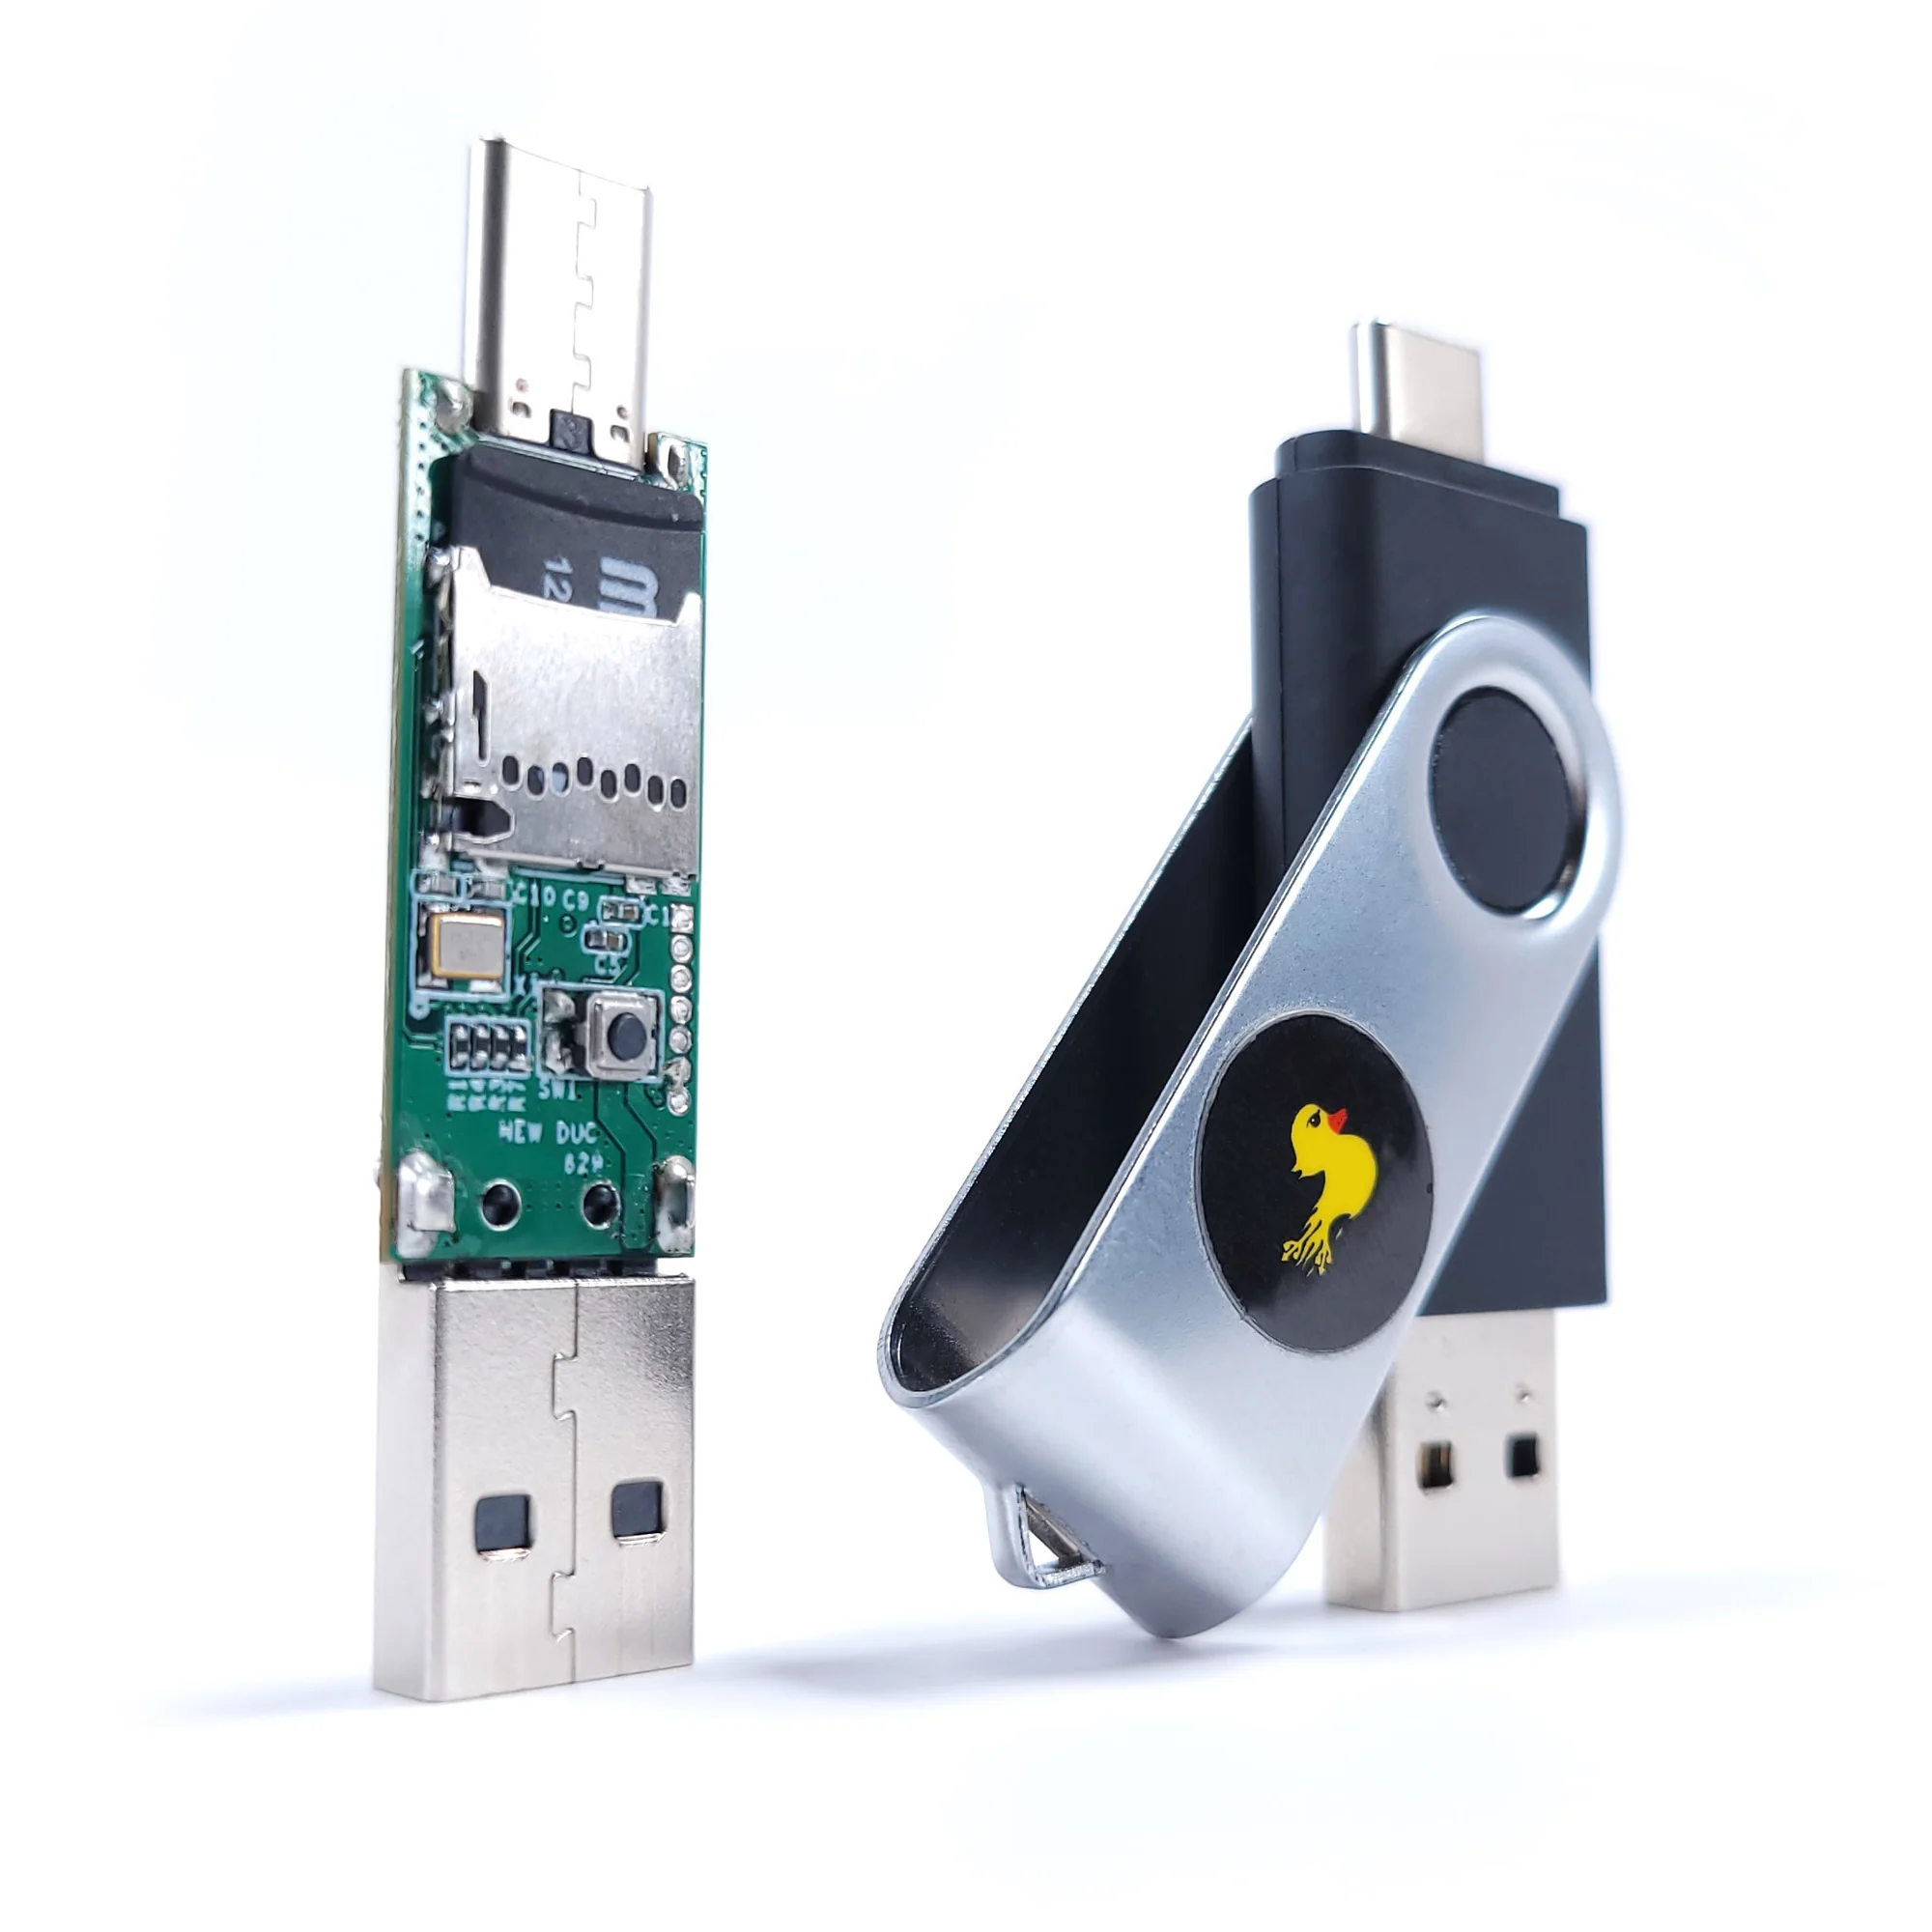
\includegraphics[alt={USB Rubber Ducky}, width=0.8\columnwidth]{img/usb-rubber-ducky_mk2_2000x.jpg}
    \caption{Dispositivo \textit{USB Rubber Ducky}.}
    Fonte: \url{https://shop.hak5.org}
    \label{fig:usb-rubber-ducky}
    \end{figure}
    \item \textbf{\textit{LAN Turtle}}, un adattatore di rete \gls{lan} che consente di instaurare accessi remoti nascosti e di analizzare il traffico direttamente dall'interno della rete aziendale. I \textit{penetration tester} utilizzano il \textit{LAN Turtle} durante le attività di \textit{penetration testing} per verificare l'esposizione delle infrastrutture a minacce derivanti dall'inserimento fisico di dispositivi malevoli;
    \begin{figure}[H]
    \centering
    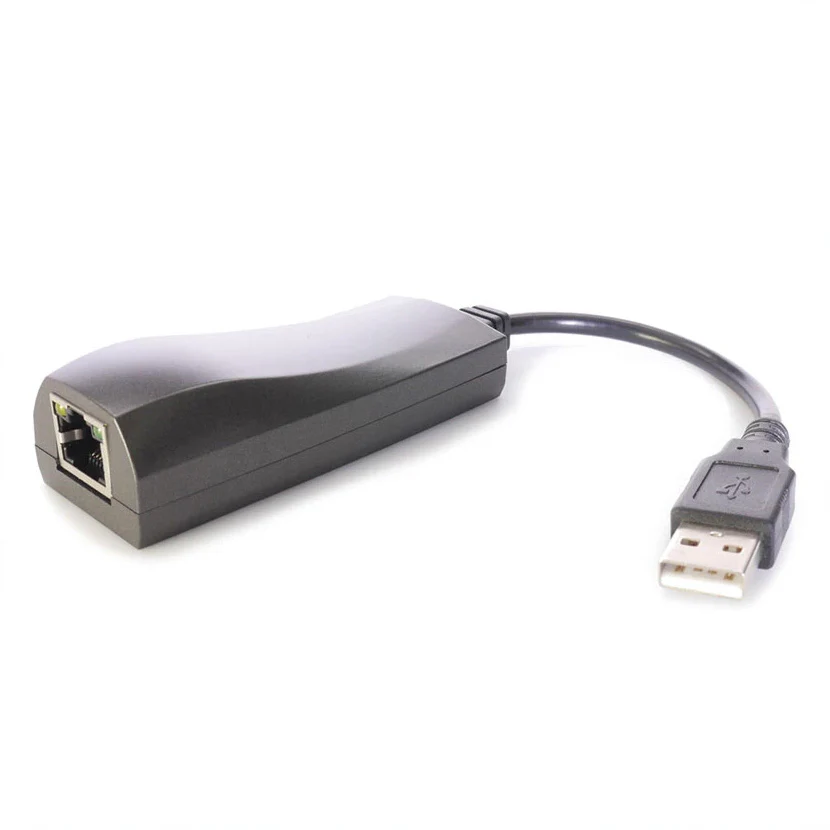
\includegraphics[alt={LAN Turtle}, width=0.8\columnwidth]{img/lan-turtle_2000x.jpg}
    \caption{Dispositivo \textit{LAN Turtle}.}
    Fonte: \url{https://shop.hak5.org}
    \label{fig:lan-turtle}
    \end{figure}
\end{itemize}
L'adozione di tali strumenti non ha un fine puramente dimostrativo, ma rappresenta un'attività concreta di valutazione del livello di sicurezza dei clienti, in quanto permette di evidenziare vulnerabilità legate al fattore umano e alla protezione fisica delle postazioni di lavoro.  
Oltre agli strumenti hardware, l'azienda analizza e adotta nuove piattaforme e metodologie orientate sia all'offensiva sia alla difensiva. Tra queste si possono citare:
\begin{itemize}
    \item l'impiego di tecniche avanzate di \textit{Threat Intelligence}, volte a raccogliere e analizzare informazioni relative a campagne malevole, infrastrutture di attacco e nuove vulnerabilità sfruttate in scenari reali;
    \item l'aggiornamento continuo dei framework di \textit{penetration testing} e \textit{vulnerability management}, che consente di disporre di strumenti più precisi ed efficaci per identificare punti deboli e priorità di intervento;
    \item la sperimentazione di approcci innovativi al \textit{red teaming}, in cui si simulano operazioni complesse di attacco, con l'obiettivo di valutare non soltanto le difese tecnologiche ma anche le capacità organizzative e di risposta dei clienti.
\end{itemize}
In conclusione, la predisposizione all'innovazione non è intesa come un'attività separata, ma come parte integrante delle operazioni quotidiane. L'integrazione di formazione, sperimentazione e ricerca applicata consente al reparto di \textit{cybersecurity} di affrontare in maniera proattiva le sfide poste dalle minacce informatiche, mantenendo un equilibrio tra lo sviluppo delle competenze interne e l'offerta di servizi sempre più efficaci e aggiornati per i clienti.


    \chapter{Scopo del progetto}
Il secondo capitolo descrive il ruolo degli \textit{stage} nel contesto aziendale e come questo abbia portato alla definizione degli obiettivi del progetto.
Inoltre vengono analizzati i vincoli e le motivazioni personali che hanno influenzato lo sviluppo del progetto stesso.

\section{Il ruolo dei tirocini in Eurosystem S.p.A.}
Eurosystem S.p.A. considera i tirocini un elemento strategico sia per la formazione dei giovani sia per l'innovazione aziendale nel settore della \textit{cybersecurity}.  
Essi permettono di avvicinarsi concretamente al mondo del lavoro e di contribuire ai progetti aziendali.  
L'azienda non interpreta il tirocinio soltanto come un'esperienza formativa, ma anche come un'opportunità per sperimentare nuove idee di progetto e per valutare soluzioni tecnologiche che, se ritenute efficaci, possono essere integrate nei servizi offerti ai clienti con l'obiettivo di rafforzarne la sicurezza informatica.  
I tirocinanti vengono accolti in un contesto lavorativo dinamico, caratterizzato da attività concrete e da un costante confronto con professionisti del settore.  
Fin dal loro inserimento, hanno la possibilità di applicare le conoscenze già acquisite e di arricchirle con competenze operative, maturate direttamente a contatto con problematiche reali della \textit{cybersecurity}.  
Questa modalità consente non solo di consolidare il proprio bagaglio tecnico, ma anche di sviluppare capacità trasversali come la collaborazione, la creatività e il \textit{problem solving}, indispensabili per affrontare scenari complessi e in continua evoluzione.  
Il tirocinio assume così un ruolo bidirezionale: da un lato favorisce la crescita formativa e professionale del tirocinante, dall'altro rappresenta per Eurosystem S.p.A. un'occasione per esplorare nuove prospettive progettuali e per individuare talenti da coinvolgere attivamente nelle sfide della sicurezza informatica.  
\section{Analisi del problema}
Uno dei principali problemi che le organizzazioni si trovano ad affrontare riguarda la capacità di \textbf{individuare tempestivamente attività malevole} all'interno dei propri sistemi.  
La sicurezza informatica rappresenta oggi una delle sfide più complesse per le aziende di qualsiasi settore. Le infrastrutture \textit{IT} moderne sono caratterizzate da un'elevata interconnessione e da una crescente dipendenza da servizi digitali, fattori che le rendono esposte a minacce sempre più sofisticate. Gli attacchi informatici non sono più episodi sporadici, ma eventi ricorrenti che possono compromettere la continuità operativa, causare perdite economiche e danneggiare in modo significativo l'azienda.\\
Le tecniche di attacco evolvono rapidamente e gli strumenti difensivi tradizionali, come \textit{firewall} e \textit{antivirus}, non sempre riescono a garantire una protezione completa. Gli operatori malevoli, infatti, sfruttano vulnerabilità sconosciute, configurazioni errate o semplicemente il fattore umano, riuscendo così ad aggirare i controlli di sicurezza.\\  
A ciò si aggiunge la difficoltà di comprendere a fondo il comportamento degli attaccanti. Spesso le aziende hanno una visibilità limitata su quali metodi vengano impiegati, su come gli aggressori si muovano una volta ottenuto l'accesso e su quali siano gli obiettivi finali delle intrusioni. Questa mancanza di informazioni rende complesso elaborare strategie di difesa realmente efficaci e impedisce di anticipare possibili minacce future.\\
In sintesi, il problema principale è legato all'\textbf{assenza di strumenti e metodologie} che consentano non solo di rilevare gli attacchi, ma anche di comprenderne le dinamiche e trarne conoscenza utile per migliorare la sicurezza complessiva dei sistemi informativi.
\begin{figure}[H]
    \begin{center}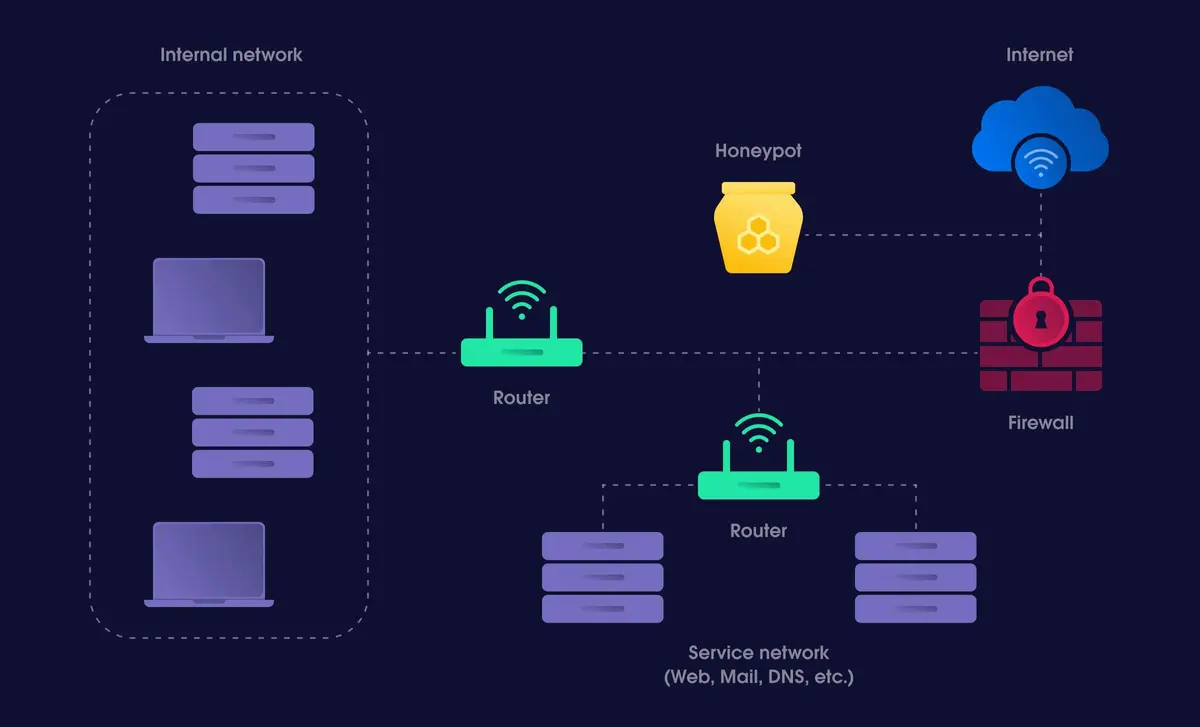
\includegraphics[alt={Honeypot position}, width=\columnwidth]{img/honeypot.jpg}
    \caption{Esempio di utilizzo di un sistema \textit{honeypot}.}
    Fonte: \url{https://oxylabs.io/blog/what-is-a-honeypot}
    \end{center}
\end{figure}
\label{fig:honeypot}
\section{Obiettivi}
Gli obiettivi che sono suddivisi in minimi, obbligatori, desiderabili o facoltativi e sono elencati di seguito.
Utilizziamo la seguente nomenclatura per suddividere questi ultimi nelle quattro tipologie:
\begin{itemize}
    \item \textbf{M}: sono gli obiettivi vincolanti e necessari per il completamento del progetto; 
    \item \textbf{O}: sono gli obiettivi primari richiesti per il progetto;
    \item \textbf{D}: sono gli obiettivi non vincolanti o strettamente necessari, ma che portano valore aggiunto al prodotto;
    \item \textbf{F}: sono gli obiettivi che portano valore aggiunto al prodotto in modo non indispensabile.
\end{itemize}
Ogni obiettivo è contrassegnato con un numero e la categoria corrispondente, al fine di garantire una classificazione chiara e ordinata.
\begin{center}
\begin{longtable}{|p{0.2\textwidth}|p{0.75\textwidth}|}
\hline
\multicolumn{1}{|c|}{\textbf{Identificativo}} & \multicolumn{1}{c|}{\textbf{Obiettivo}}\\ 
\hline 
\endfirsthead
\multicolumn{2}{c}{{\bfseries \tablename\ \thetable{} -- Continuo della tabella}}\\
\hline
\multicolumn{1}{|c|}{\textbf{Identificativo}} & \multicolumn{1}{c|}{\textbf{Obiettivo}}\\ \hline 
\endhead
\hline
\multicolumn{2}{|r|}{{Continua nella prossima pagina...}}\\
\hline
\endfoot
\endlastfoot 

\multicolumn{2}{|c|}{\textbf{Obiettivi Minimi}} \\ \hline
M01 & Il codice del progetto deve essere scritto in \textit{Python}, deve avere struttura modulare e commenti esplicativi. \\ \hline
M02 & Il progetto deve presentare configurazioni leggibili, versionate e testate. \\ \hline
M03 & Gli \textit{script} devono essere riutilizzabili e gli \textit{input} devono essere parametrizzabili. \\ \hline
M04 & Il progetto deve avere una documentazione coerente con quanto implementato, scritta in forma tecnica, chiara e verificabile. \\ \hline

\multicolumn{2}{|c|}{\textbf{Obiettivi Obbligatori}} \\ \hline
O01 & Deve essere installata e configurata una macchina virtuale isolata per ambienti \textit{honeypot}. \\ \hline
O02 & L'\textit{honeypot} prodotto deve essere realistico con configurazione di servizi vulnerabili (\textit{Apache}, \gls{ftp}\glsadd{ftp_def}, \gls{smb}\glsadd{smb_def}, \gls{mqtt}, ecc.). \\ \hline
O03 & Devono essere sviluppati servizi \textit{dummy} con \textit{netcat} o strumenti equivalenti per l'ascolto dei pacchetti. \\ \hline
O04 & I \textit{log} devono essere raccolti e centralizzati tramite \textit{Python} e \textit{pipeline} \gls{tig}. \\ \hline
O05 & La raccolta dei \textit{log} deve essere automatizzata mediante \textit{script} \textit{Python}/\textit{Bash}. \\ \hline

\multicolumn{2}{|c|}{\textbf{Obiettivi Desiderabili}} \\ \hline
D01 & Deve essere effettuata un'analisi tecnica degli attacchi ricevuti con relativa correlazione dei dati. \\ \hline
D02 & Devono essere integrati strumenti e tecniche di \textit{Threat Intelligence} e \gls{osint}\glsadd{osint_def} per finalità di attribuzione. \\ \hline
D03 & Devono essere simulati attacchi controllati con strumenti noti e devono essere raccolti i relativi \textit{output}. \\ \hline
D04 & Devono essere applicate tecniche di base di \textit{data analysis} per il riconoscimento di \textit{pattern}. \\ \hline
D05 & Deve essere realizzata una \textit{dashboard} con grafici, \gls{ioc}\glsadd{ioc_def} e \textit{timeline} degli eventi. \\ \hline

\multicolumn{2}{|c|}{\textbf{Obiettivi Facoltativi}} \\ \hline
F01 & Devono essere implementati controlli avanzati di \textit{audit} con \textit{auditd} e \textit{logging} \textit{Bash} persistente. \\ \hline
F02 & Deve essere sperimentata la distribuzione dei dati verso \gls{siem}\glsadd{siem_def} \textit{open source}. \\ \hline
F03 & Devono essere introdotti strumenti di \gls{ai}/\gls{ml} per l'identificazione automatica di anomalie. \\ \hline

\caption{Elenco degli obiettivi suddivisi per categoria.}
\label{tab:obiettivi}
\end{longtable}
\end{center}

\section{Vincoli}
Durante lo sviluppo del progetto non sono stati imposti particolari vincoli di tipo architetturale, ma sono emersi alcuni vincoli tecnologici, progettuali, metodologici e temporali che hanno orientato le scelte di implementazione. 
\subsection{Vincoli tecnologici}
Dal punto di vista tecnologico, è stato imposto l'utilizzo di \textbf{\textit{Python}} (v.3.12.10) come linguaggio di programmazione. Questa scelta è stata dettata non solo dalla sua versatilità e dalla disponibilità di numerose librerie utili allo sviluppo, ma anche perché rappresenta uno dei linguaggi più diffusi nell'ambito della \textit{cybersecurity}, oltre a essere quello su cui l'azienda possiede maggiore esperienza interna. Per la gestione e la visualizzazione dei dati si è optato per lo \textit{stack \textbf{TIG}}, composto da \textit{Telegraf} (v.1.24), \textit{InfluxDB} (v.2.7) e \textit{Grafana} (v.9.5.6), preferito al più diffuso \textit{stack} \gls{elk} per la sua leggerezza e per la maggiore aderenza ai requisiti del progetto. Anche le modalità di comunicazione tra i diversi componenti sono state soggette a vincolo: è stato infatti imposto l'uso del protocollo \textit{\textbf{MQTT}}, particolarmente adatto allo scambio di dati in tempo reale con un consumo ridotto di risorse. Al contrario, non sono stati previsti vincoli riguardo ai servizi vulnerabili da esporre all'interno del sistema \textit{honeypot}, lasciando piena libertà di scelta in base alle esigenze di implementazione. 
Sul piano progettuale, è stato stabilito che il sistema dovesse includere un \textit{logger} interno. Questo vincolo ha avuto un impatto diretto sulla progettazione complessiva, in quanto ha reso necessaria l'integrazione di meccanismi di \textit{logging} fin dalle fasi iniziali, in modo da facilitare il \textit{debugging} durante lo sviluppo.
\begin{figure}[H]
    \centering
    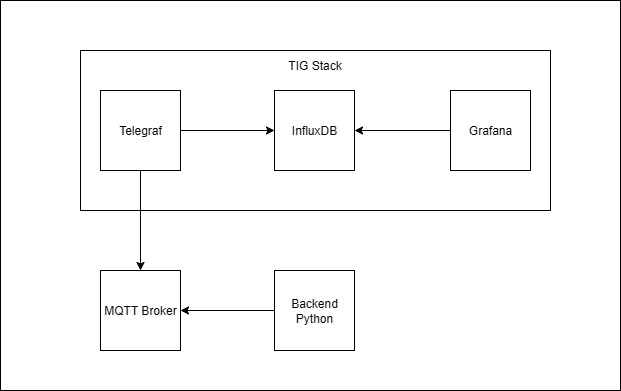
\includegraphics[alt={Schema MQTT-TIG}, width=\columnwidth]{img/mqtt-tig.png}
    \caption{Schema di esempio dell'integrazione tra protocollo \textit{MQTT} e \textit{stack} \textit{TIG}.}
    \label{fig:mqtt-tig}
\end{figure}
\subsection{Vincoli metodologici}
Per quanto concerne la metodologia, il progetto è stato strutturato in quattro fasi principali, che hanno guidato sia la pianificazione sia l'esecuzione: 
\begin{itemize}
    \item \textbf{Fase 1 (Setup dell'ambiente)}: predisposizione di un contesto sicuro e, al tempo stesso, sufficientemente vulnerabile per ospitare \textit{honeypot} e servizi di interesse;
    \item \textbf{Fase 2 (Sviluppo del \textit{logger} e installazione della pipeline \textit{TIG})}: costruzione di una \textit{pipeline} di raccolta, gestione e visualizzazione dei dati, con particolare attenzione alla scalabilità;
    \item \textbf{Fase 3 (Setup della \textit{data analysis})}: implementazione di strumenti e metodologie per l'analisi e la correlazione dei dati, finalizzati al miglioramento dei processi di rilevazione e risposta agli attacchi;
    \item \textbf{Fase 4 (Attesa o simulazione di attacchi e redazione dei \textit{report})}: osservazione delle interazioni con il sistema e produzione di \textit{report} operativi a supporto dell'analisi.
\end{itemize}
\subsection{Vincoli temporali}
Infine, relativamente ai vincoli temporali, l'unico vincolo significativo era rappresentato dalla durata del tirocinio, pari a due mesi. L'avanzamento delle diverse fasi è dunque dipeso in larga misura dalla rapidità con cui è stato possibile apprendere e applicare le competenze necessarie, rendendo il fattore tempo un elemento variabile e fortemente legato alla curva di apprendimento individuale.


\section{Prospettive future}
Sono presenti diverse possibilità di evoluzione, finalizzate a incrementarne le funzionalità e l'efficacia del progetto. 
Una possibile estensione riguarda l'aggiunta di ulteriori servizi vulnerabili nel sistema \textit{honeypot}, con l'obiettivo di renderlo più realistico e in grado di raccogliere un numero maggiore di dati sulle tecniche di attacco.  
Si potrebbe inoltre rendere il sistema esposto alla rete, rimuovendo alcune limitazioni imposte dai \textit{firewall}, in modo da osservare interazioni più eterogenee con l'ambiente esterno e analizzare comportamenti degli attaccanti più complessi.  
Un'ulteriore evoluzione riguarda l'introduzione di meccanismi automatici per l'identificazione delle anomalie, sfruttando strumenti di \textit{AI} e \textit{ML}. Questo permetterebbe di automatizzare il rilevamento delle minacce e di ridurre i tempi di risposta agli attacchi.  
È inoltre possibile estendere il sistema di \textit{logging} per supportare più lingue, migliorando l'usabilità e la fruibilità dei dati da parte di \textit{team} internazionali o utenti non madrelingua.  
Infine, il progetto potrebbe essere reso un pacchetto unico distribuibile ai clienti, semplificando l'installazione e la configurazione del sistema e favorendone l'adozione in contesti differenti.  
Queste evoluzioni rappresentano opportunità concrete per aumentare il valore del sistema e garantirne una maggiore flessibilità, automatizzazione e facilità d'uso.

\section{Motivazioni personali}
Descrive le motivazioni personali che hanno spinto alla scelta di questo stage, gli interessi specifici nel campo della \textit{cybersecurity} e le aspettative di crescita professionale.
    \chapter{Sviluppo del progetto}
Il terzo capitolo illustra gli strumenti, le tecnologie e le metodologie adottate, descrivendo come siano state applicate e presentando un quadro generale dello svolgimento del progetto: dall'analisi delle richieste aziendali, fino allo sviluppo del prodotto finale. 
\keepXColumns
\section{Analisi dei requisiti}
La fase di \textbf{analisi dei requisiti} consiste nello studio e nell'esame delle esigenze espresse dall'azienda, con l'obiettivo di definire in modo preciso e completo i requisiti del sistema.  
Questa parte del progetto si è svolta nell'arco di due settimane, durante le quali ho organizzato incontri regolari con il tutor aziendale per confrontarsi su progressi, criticità e possibili soluzioni. Le principali attività condotte includono:
\begin{itemize}
    \item \textbf{Sessioni di \textit{brainstorming}} con il tutor, finalizzate alla definizione degli obiettivi e delle priorità del sistema;
    \item \textbf{Studio della documentazione} di sistemi \textit{honeypot} esistenti, per comprendere metodologie consolidate e funzionalità tipiche;
    \item \textbf{Analisi delle \textit{best practice}} in ambito \textit{cybersecurity} per sistemi \textit{ETL}, a garanzia di sicurezza e affidabilità;
    \item \textbf{Valutazione dei vincoli tecnologici} imposti dall'ambiente aziendale, tra cui piattaforme disponibili, linguaggi di programmazione e strumenti di monitoraggio.
\end{itemize}
Dall'analisi effettuata sono emersi i \hyperref[casi-uso]{casi d'uso} sulla quale si è basato il progetto.
\subsection{Casi d'uso}
\label{casi-uso}
I \textbf{casi d'uso} descrivono una funzionalità specifica che il sistema deve fornire a uno o più attori (che possono essere utenti o altri sistemi), indicando le interazioni e i risultati ottenuti dal punto di vista degli attori.
Per sviluppare i casi d'uso abbiamo utilizzato il linguaggio \gls{uml}\glsadd{uml_def}, uno strumento di modellazione che mostra le interazioni tra attori e casi d'uso attraverso relazioni come \textit{<<include>>}, \textit{<<extend>>} e generalizzazioni.
La seguente convenzione di nomenclatura supporta l'identificazione dei casi d'uso e ne facilita l'organizzazione e la tracciabilità:\\
\begin{center}
\textbf{UC.ID.subID}
\end{center}
\begin{itemize}
    \item \textbf{UC}: è l'identificatore dei casi d'uso;
    \item \textbf{ID}: è l'identificatore numerico del caso d'uso principale;
    \item \textbf{subID}: è l'identificatore numerico dei sotto-casi d'uso che specifica i casi d'uso associati a un caso d'uso principale.
\end{itemize}
\begin{figure}[H]
    \begin{center}
        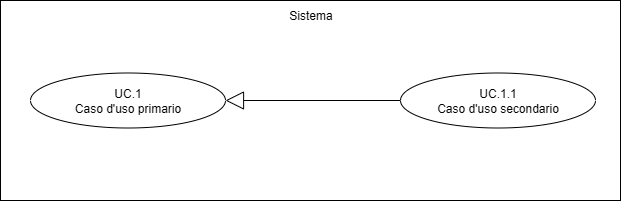
\includegraphics[alt={Esempio di caso d'uso e sotto-caso d'uso}, width=0.8\columnwidth]{img/esempio_uc.png}
        \caption{Esempio di caso d'uso e sotto-caso d'uso.}
        \label{fig:es-uc}
    \end{center}
\end{figure}
\subsection*{Attori dei casi d'uso}
Nel contesto dei casi d'uso, gli attori del sistema si suddividono in due categorie principali: \textbf{attori primari} e \textbf{attori secondari}.\\\\
Gli \textbf{attori primari} sono coloro che avviano attivamente un caso d'uso con l'obiettivo di ottenere un risultato specifico attraverso l'interazione diretta con il sistema. Rappresentano gli utenti o le entità che traggono un beneficio concreto dall'esecuzione del caso d'uso.\\
All'interno del progetto l'attore principale è:
\begin{itemize}
    \item \textbf{Utente}: cioè un utente membro del team di \textit{cybersecurity} che ha accesso all'\textit{honeypot}.
\end{itemize}
Al contrario, gli \textbf{attori secondari} non iniziano il caso d'uso, ma forniscono supporto o servizi necessari affinché il sistema possa completarlo correttamente. Interagiscono in modo indiretto o passivo, contribuendo al funzionamento del processo senza esserne i promotori principali. In questo caso all'interno del sistema non sono presenti attori secondari, poiché non ci sono entità che svolgono un ruolo di supporto indiretto al processo.\\
\begin{figure}[H]
    \begin{center}
        
\includegraphics[alt={Esempio di attore}, width=0.075\columnwidth]{img/attore.png}
        \caption{Esempio di attore.}
        \label{fig:es-attore}
    \end{center}
\end{figure}
\subsubsection*{Lista dei casi d'uso}
Di seguito si trovano i casi d'uso principali del sistema.
Non sono riportati tutti i casi d'uso individuati in fase di analisi, ma soltanto quelli ritenuti maggiormente rappresentativi e funzionali alla comprensione delle caratteristiche essenziali del sistema.
La scelta di limitarne il numero risponde a due esigenze: da un lato evitare ridondanze o descrizioni eccessivamente dettagliate di funzionalità marginali, dall'altro garantire una visione chiara e sintetica delle capacità chiave del sistema in relazione ai suoi obiettivi progettuali.
\begin{center}
\begin{longtable}{|p{0.3\textwidth}|p{0.65\textwidth}|}
\hline
\multicolumn{2}{|c|}{\textbf{UC.1}}\\ 
\hline 
\endfirsthead
\multicolumn{2}{c}{{\bfseries \tablename\ \thetable{} -- Continuo della tabella}}\\
\hline
\multicolumn{2}{|c|}{\textbf{UC.1}}\\ \hline 
\endhead
\hline
\multicolumn{2}{|r|}{{Continua nella prossima pagina...}}\\
\hline
\endfoot
\endlastfoot
% Riga immagine che occupa entrambe le colonne
\multicolumn{2}{|c|}{
    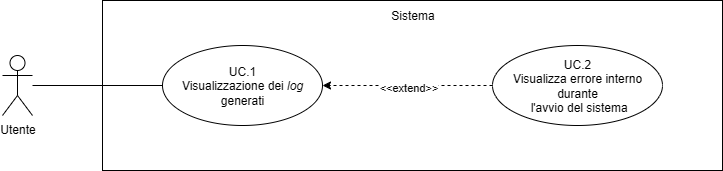
\includegraphics[width=\textwidth]{img/UC-1.png}
}\\ \hline
\textbf{Pre-condizioni} & Il sistema è attivo e funzionante. \\ \hline
\textbf{Post-condizioni} & Vengono visualizzati i \textit{log} generati dal sistema \textit{honeypot}. \\ \hline
\textbf{Attori principali} & Utente \\ \hline
\textbf{Scenario principale} & 
\begin{itemize}
    \item L'utente richiede la visualizzazione dei \textit{log} del sistema;
    \item Il sistema verifica la presenza e la conformità dei \textit{log};
    \item I dati del sistema vengono visualizzati in ordine cronologico di creazione.
\end{itemize} \\ \hline
\textbf{Scenario secondario} & 
\begin{itemize}
    \item Si verifica un errore interno durante l'avvio del sistema che impedisce la visualizzazione dei \textit{log} (\hyperref[tab:uc-2]{UC.2}).
\end{itemize} \\ \hline
\caption{Diagramma del caso d'uso UC.1 - Visualizzare i \textit{log} del sistema \textit{honeypot}.}
\label{tab:uc-1}
\end{longtable}
\end{center}

\begin{center}
\begin{longtable}{|p{0.3\textwidth}|p{0.65\textwidth}|}
\hline
\multicolumn{2}{|c|}{\textbf{UC.2}}\\ 
\hline 
\endfirsthead
\multicolumn{2}{c}{{\bfseries \tablename\ \thetable{} -- Continuo della tabella}}\\
\hline
\multicolumn{2}{|c|}{\textbf{UC.2}}\\ \hline 
\endhead
\hline
\multicolumn{2}{|r|}{{Continua nella prossima pagina...}}\\
\hline
\endfoot
\endlastfoot
% Riga immagine che occupa entrambe le colonne
\textbf{Pre-condizioni} & L'avvio delle diverse componenti del sistema non avviene correttamente. \\ \hline
\textbf{Post-condizioni} & L'utente visualizza gli errori che impediscono l'avvio del sistema e il loro livello di gravità. \\ \hline
\textbf{Attori principali} & Utente \\ \hline
\textbf{Scenario principale} & 
\begin{itemize}
    \item L'utente avvia il sistema;
    \item Il sistema verifica lo stato delle sue componenti;
    \item Se si verifica un errore, il sistema comunica all'utente quale componente non si è avviata correttamente.
\end{itemize} \\ \hline
\textbf{Scenario secondario} & 
\begin{itemize}
    \item N/A 
\end{itemize} \\ \hline
\caption{Diagramma del caso d'uso UC.2 - Visualizza errore interno durante l'avvio del sistema.}
\label{tab:uc-2}
\end{longtable}
\end{center}

\begin{center}
\begin{longtable}{|p{0.3\textwidth}|p{0.65\textwidth}|}
\hline
\multicolumn{2}{|c|}{\textbf{UC.3}}\\ 
\hline 
\endfirsthead
\multicolumn{2}{c}{{\bfseries \tablename\ \thetable{} -- Continuo della tabella}}\\
\hline
\multicolumn{2}{|c|}{\textbf{UC.3}}\\ \hline 
\endhead
\hline
\multicolumn{2}{|r|}{{Continua nella prossima pagina...}}\\
\hline
\endfoot
\endlastfoot
% Riga immagine che occupa entrambe le colonne
\multicolumn{2}{|c|}{
    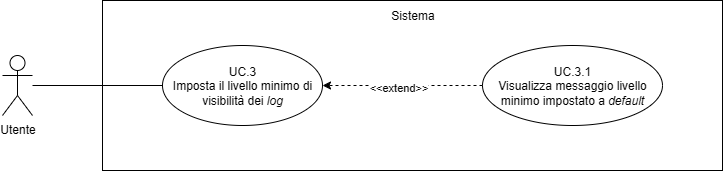
\includegraphics[width=\textwidth]{img/UC-3.png}
}\\ \hline
\textbf{Pre-condizioni} & Il sistema è in fase di avvio. \\ \hline
\textbf{Post-condizioni} & Il livello minimo dei \textit{log} da visualizzare è impostato. \\ \hline
\textbf{Attori principali} & Utente \\ \hline
\textbf{Scenario principale} & 
\begin{itemize}
    \item L'utente visualizza i possibili livelli minimi del sistema;
    \item L'utente seleziona il livello minimo desiderato;
    \item Il sistema applica la nuova configurazione e conferma l'avvenuta modifica.
\end{itemize} \\ \hline
\textbf{Scenario secondario} & 
\begin{itemize}
    \item L'utente seleziona un livello non valido, oppure non seleziona nessun livello.
\end{itemize} \\ \hline
\caption{Diagramma del caso d'uso UC.3 - Impostare il livello minimo dei \textit{log} da visualizzare.}
\label{tab:uc-3}
\end{longtable}
\end{center}

\begin{center}
\begin{longtable}{|p{0.3\textwidth}|p{0.65\textwidth}|}
\hline
\multicolumn{2}{|c|}{\textbf{UC.4}}\\ 
\hline 
\endfirsthead
\multicolumn{2}{c}{{\bfseries \tablename\ \thetable{} -- Continuo della tabella}}\\
\hline
\multicolumn{2}{|c|}{\textbf{UC.4}}\\ \hline 
\endhead
\hline
\multicolumn{2}{|r|}{{Continua nella prossima pagina...}}\\
\hline
\endfoot
\endlastfoot
% Riga immagine che occupa entrambe le colonne
\multicolumn{2}{|c|}{
    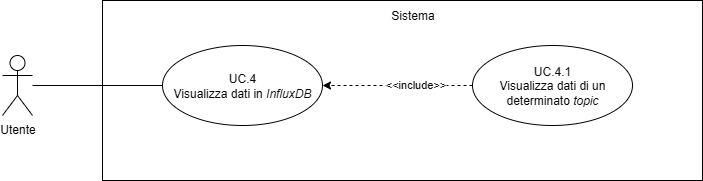
\includegraphics[width=\textwidth]{img/UC-4.png}
}\\ \hline
\textbf{Pre-condizioni} & Il sistema è attivo e funzionante. \\ \hline
\textbf{Post-condizioni} & Vengono visualizzati i dati presenti in \textit{InfluxDB}. \\ \hline
\textbf{Attori principali} & Utente \\ \hline
\textbf{Scenario principale} & 
\begin{itemize}
    \item L'utente richiede la visualizzazione dei dati presenti in \textit{InfluxDB};
    \item Il sistema verifica la presenza e la conformità dei dati;
    \item I dati presenti in \textit{InfluxDB} vengono visualizzati in base ai filtri selezionati.
\end{itemize} \\ \hline
\textbf{Scenario secondario} & 
\begin{itemize}
    \item Non sono presenti dati in \textit{InfluxDB} da visualizzare;
    \item Il sistema non mostra alcun dato all'utente.
\end{itemize} \\ \hline
\caption{Diagramma del caso d'uso UC.4 - Visualizzare i dati presenti in \textit{InfluxDB}.}
\label{tab:uc-4}
\end{longtable}
\end{center}

\begin{center}
\begin{longtable}{|p{0.3\textwidth}|p{0.65\textwidth}|}
\hline
\multicolumn{2}{|c|}{\textbf{UC.5}}\\ 
\hline 
\endfirsthead
\multicolumn{2}{c}{{\bfseries \tablename\ \thetable{} -- Continuo della tabella}}\\
\hline
\multicolumn{2}{|c|}{\textbf{UC.5}}\\ \hline 
\endhead
\hline
\multicolumn{2}{|r|}{{Continua nella prossima pagina...}}\\
\hline
\endfoot
\endlastfoot
% Riga immagine che occupa entrambe le colonne
\multicolumn{2}{|c|}{
    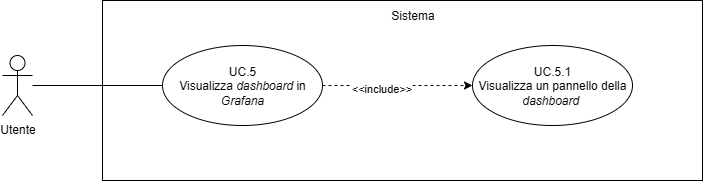
\includegraphics[width=\textwidth]{img/UC-5.png}
}\\ \hline
\textbf{Pre-condizioni} & Il sistema è attivo e funzionante. \\ \hline
\textbf{Post-condizioni} & Viene visualizzata una \textit{dashboard} in \textit{Grafana}. \\ \hline
\textbf{Attori principali} & Utente \\ \hline
\textbf{Scenario principale} & 
\begin{itemize}
    \item L'utente richiede la visualizzazione di una \textit{dashboard} in \textit{Grafana};
    \item Il sistema verifica la presenza e la conformità della \textit{dashboard};
    \item La \textit{dashboard} viene visualizzata con i dati aggiornati in tempo reale.
\end{itemize} \\ \hline
\textbf{Scenario secondario} & 
\begin{itemize}
    \item Non sono presenti dati in \textit{InfluxDB} da visualizzare;
    \item Il sistema non mostra alcun dato all'utente.
\end{itemize} \\ \hline
\caption{Diagramma del caso d'uso UC.5 - Visualizzare una \textit{dashboard} in \textit{Grafana}.}
\label{tab:uc-5}
\end{longtable}
\end{center}

\begin{center}
\begin{longtable}{|p{0.3\textwidth}|p{0.65\textwidth}|}
\hline
\multicolumn{2}{|c|}{\textbf{UC.6}}\\ 
\hline 
\endfirsthead
\multicolumn{2}{c}{{\bfseries \tablename\ \thetable{} -- Continuo della tabella}}\\
\hline
\multicolumn{2}{|c|}{\textbf{UC.6}}\\ \hline 
\endhead
\hline
\multicolumn{2}{|r|}{{Continua nella prossima pagina...}}\\
\hline
\endfoot
\endlastfoot
% Riga immagine che occupa entrambe le colonne
\multicolumn{2}{|c|}{
    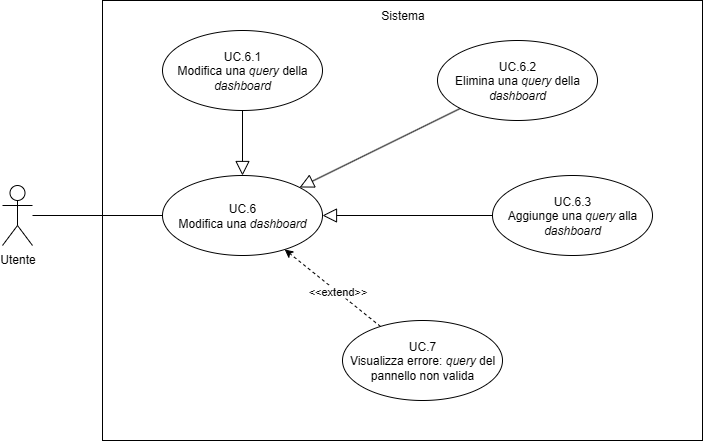
\includegraphics[width=\textwidth]{img/UC-6.png}
}\\ \hline
\textbf{Pre-condizioni} & Il sistema è attivo e funzionante. \\ \hline
\textbf{Post-condizioni} & Viene modificata una \textit{dashboard} in \textit{Grafana}. \\ \hline
\textbf{Attori principali} & Utente \\ \hline
\textbf{Scenario principale} & 
\begin{itemize}
    \item L'utente modifica una \textit{dashboard} in \textit{Grafana};
    \item Il sistema verifica la conformità della \textit{query};
    \item La \textit{dashboard} viene aggiornata con le nuove impostazioni.
\end{itemize} \\ \hline
\textbf{Scenario secondario} & 
\begin{itemize}
    \item La modifica non è conforme agli standard di \textit{Grafana} (\hyperref[tab:uc-7]{UC.7}).
\end{itemize} \\ \hline
\caption{Diagramma del caso d'uso UC.6 - Modificare una \textit{dashboard} in \textit{Grafana}.}
\label{tab:uc-6}
\end{longtable}
\end{center}

\begin{center}
\begin{longtable}{|p{0.3\textwidth}|p{0.65\textwidth}|}
\hline
\multicolumn{2}{|c|}{\textbf{UC.7}}\\ 
\hline 
\endfirsthead
\multicolumn{2}{c}{{\bfseries \tablename\ \thetable{} -- Continuo della tabella}}\\
\hline
\multicolumn{2}{|c|}{\textbf{UC.7}}\\ \hline 
\endhead
\hline
\multicolumn{2}{|r|}{{Continua nella prossima pagina...}}\\
\hline
\endfoot
\endlastfoot
\textbf{Pre-condizioni} & La modifica effettuata dall'utente non è valida. \\ \hline
\textbf{Post-condizioni} & Viene visualizzato il pannello di errore. \\ \hline
\textbf{Attori principali} & Utente \\ \hline
\textbf{Scenario principale} & 
\begin{itemize}
    \item L'utente modifica una \textit{dashboard} in \textit{Grafana};
    \item Il sistema verifica la conformità della modifica effettuata;
    \item La modifica non è conforme agli standard di \textit{Grafana};
    \item Il sistema visualizza il pannello di errore.
\end{itemize} \\ \hline
\textbf{Scenario secondario} & 
\begin{itemize}
    \item N/A
\end{itemize} \\ \hline
\caption{Diagramma del caso d'uso UC.7 - Visualizza errore: \textit{query} del pannello non valida.}
\label{tab:uc-7}
\end{longtable}
\end{center}
\subsection{Requisiti}
\label{requisiti}
I requisiti si dividono in tre categorie principali: funzionali, non funzionali e di vincolo, che specificano rispettivamente cosa deve fare il sistema, come deve funzionare e quali condizioni deve rispettare per operare. 
I primi sono le azioni che il sistema deve compiere, mentre i secondi sono le qualità che deve avere (come la velocità o la sicurezza). 
I requisiti di vincolo, invece, riguardano le restrizioni imposte al sistema, come la piattaforma su cui deve girare o il linguaggio di programmazione da utilizzare. 
In seguito alla definizione dei casi d'uso, ho quindi identificato e documentato i requisiti funzionali, non funzionali e di vincolo del sistema.
La determinazione di tali requisiti è avvenuta assieme al tutor aziendale e sono alla base della progettazione e dello sviluppo.

\subsubsection*{Requisiti funzionali}
\begin{itemize}[noitemsep, topsep=0pt]
    \item RF.1: Raccogliere automaticamente i \textit{log} generati dai servizi \textit{honeypot}.
    \item RF.2: Centralizzare i \textit{log} raccolti in un \textit{database} (\textit{InfluxDB}).
    \item RF.3: Visualizzare i \textit{log} in tempo reale attraverso un'interfaccia o strumento di monitoraggio.
    \item RF.4: Consentire la configurazione del livello minimo di \textit{log} da mostrare.
    \item RF.5: Reimpostare il livello minimo di \textit{log} al valore predefinito e notificare l'utente.
    \item RF.6: Segnalare errori interni durante l'avvio del sistema.
    \item RF.7: Visualizzare i dati salvati in \textit{InfluxDB} tramite \textit{Grafana}.
    \item RF.8: Creare e modificare \textit{dashboard} in \textit{Grafana}.
    \item RF.9: Aggiungere, modificare ed eliminare \textit{query} nelle \textit{dashboard}.
    \item RF.10: Mostrare errori in caso di \textit{query} non valida nei pannelli \textit{Grafana}.
    \item RF.11: Simulare attacchi controllati e raccoglierne i \textit{log}.
    \item RF.12: Fornire \textit{dashboard} avanzate con grafici, \textit{IOC} e \textit{timeline} degli eventi.
    \item RF.13: Esportare i dati verso \textit{SIEM} \textit{open source}.
\end{itemize}

\subsubsection*{Requisiti non funzionali}
\begin{itemize}[noitemsep, topsep=0pt]
    \item RNF.1: Modularità del codice per favorire estendibilità e manutenzione.
    \item RNF.2: Documentazione tecnica chiara, verificabile e coerente con il codice.
    \item RNF.3: Commenti esplicativi nel codice per facilitarne la comprensione.
    \item RNF.4: Riutilizzabilità degli \textit{script} e parametrizzazione degli \textit{input}.
    \item RNF.5: Configurazioni del codice leggibili, versionate e testate.
    \item RNF.6: Sicurezza nell'accesso ai \textit{log} e alle \textit{dashboard} tramite autenticazione.
    \item RNF.7: Persistenza dei dati raccolti per consentire analisi storiche.
    \item RNF.8: Scalabilità per aggiungere nuovi servizi \textit{honeypot} o \textit{pipeline} senza modifiche invasive.
    \item RNF.9: Affidabilità nella raccolta dei \textit{log} (nessuna perdita di dati in caso di errore temporaneo).
    \item RNF.10: Chiarezza dei messaggi di errore, comprensibili anche a utenti non tecnici.
\end{itemize}

\subsubsection*{Requisiti di vincolo}
\begin{itemize}[noitemsep, topsep=0pt]
    \item RV.1: Esecuzione in una macchina virtuale isolata per motivi di sicurezza.
    \item RV.2: Utilizzo del linguaggio di programmazione \textit{Python}.
    \item RV.3: Utilizzo della \textit{pipeline TIG}.
    \item RV.4: Presenza di servizi vulnerabili realistici da esporre nel sistema \textit{honeypot}.
    \item RV.5: Uso di servizi \textit{dummy} con \textit{netcat} o strumenti equivalenti per simulare ascolto pacchetti.
    \item RV.6: Raccolta \textit{log} automatizzata mediante \textit{script Python} o \textit{Bash}.
    \item RV.7: Gestione di configurazioni e codice tramite sistemi di versionamento (es. \textit{Git}).
\end{itemize}
Infine, la seguente tabella riassume durata, \textit{output} e metriche delle attività di analisi dei requisiti:
\begin{center}
\begin{longtable}{|p{0.35\textwidth}|p{0.15\textwidth}|p{0.25\textwidth}|p{0.2\textwidth}|}
\hline
\multicolumn{1}{|c|}{\textbf{Attività}} & 
\multicolumn{1}{c|}{\textbf{Durata}} & 
\multicolumn{1}{c|}{\textbf{Prodotti}} & 
\multicolumn{1}{c|}{\textbf{Metriche}} \\ 
\hline
\endfirsthead

\multicolumn{4}{c}{{\bfseries \tablename\ \thetable{} -- Continuo della tabella}}\\
\hline
\multicolumn{4}{|c|}{\textbf{Attività di analisi condotte}} \\ \hline
\endhead

\hline \multicolumn{4}{|r|}{{Continua nella prossima pagina...}} \\ \hline
\endfoot

\endlastfoot

Sessioni di \textit{brainstorming} col tutor & 2 settimane & 11 casi d'uso definiti & 8 incontri da 1 ora ciascuno \\ \hline
Studio documentazione honeypot esistenti & 1 settimana & Relazione interna & 15 sistemi analizzati \\ \hline
Analisi \textit{best practice ETL cybersecurity} & 3 giorni & Relazione interna & 12 framework valutati \\ \hline
Definizione requisiti funzionali & 2 giorni & 13 requisiti RF & 2 iterazioni di revisione \\ \hline
Definizione requisiti non funzionali & 1 giorno & 10 requisiti RNF & 2 iterazioni di revisione \\ \hline
Definizione requisiti di vincolo & 1 giorno & 7 requisiti RV & 2 iterazioni di revisione \\ \hline

\caption{Tabella quantitativa dell'analisi dei requisiti.}
\label{tab:tempistiche-analisi}
\end{longtable}
\end{center}
\section{Progettazione}
\subsection{Architettura del sistema}
Per questo progetto, essendo fondamentalmente un sistema \gls{etl}\glsadd{etl_def} ho deciso di adottare un'architettura a più livelli, che consente di separare le diverse funzionalità del sistema in moduli distinti e indipendenti.
Il primo livello è rappresentato dai servizi \textit{honeypot}, che simulano i servizi di rete vulnerabili e raccolgono i \textit{log} delle attività sospette.
Il secondo livello è costituito dai \textit{script} di raccolta e trasferimento dei \textit{log}, che elaborano i dati raccolti e li inviano al database.
Il terzo livello è rappresentato dal \textit{database} \textit{InfluxDB}, che memorizza i \textit{log} in modo strutturato e consente di eseguire query sui dati.
Infine, i dati vengono visualizzati tramite \textit{Grafana}, che offre un'interfaccia intuitiva per l'analisi e la visualizzazione delle informazioni.
\begin{figure}[H]
    \begin{center}
    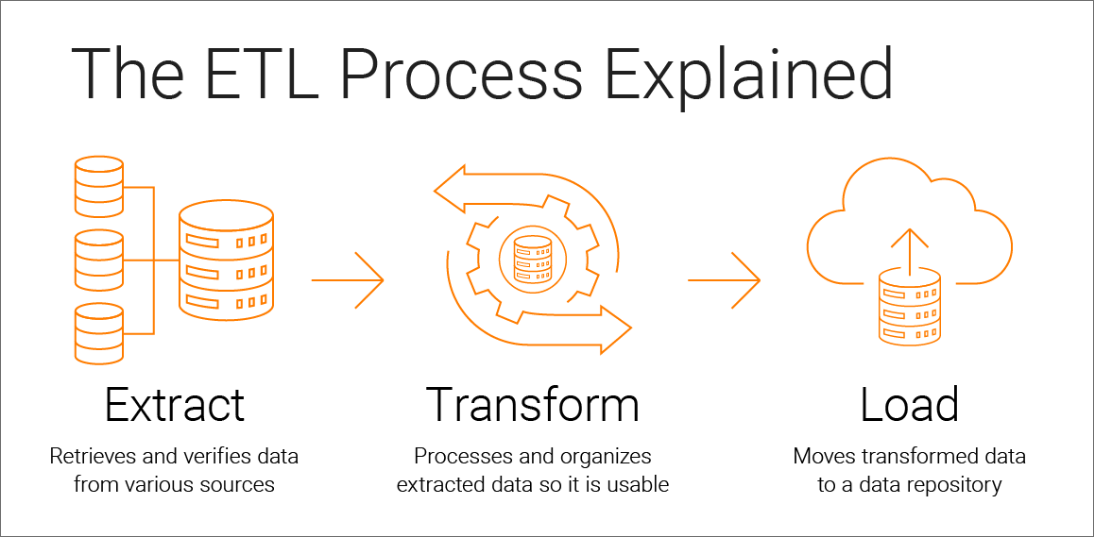
\includegraphics[width=0.9\textwidth]{img/etl-process-explained-diagram.png}
    \caption{Architettura del sistema \textit{ETL}.}
    Fonte: \url{https://www.informatica.com/resources/articles/what-is-etl.html}
    \label{fig:etl-architecture}
    \end{center}
\end{figure}
Partendo da questa architettura di base, ho progettato il sistema in maniera tale da essere modulare e scalabile, in modo da poter aggiungere facilmente nuovi servizi vulnerabili al sistema \textit{honeypot} o modificare quelli esistenti senza influire sulle altre componenti.
Ho quindi prodotto il seguente diagramma di flusso che rappresenta il funzionamento generale del prodotto, dalla raccolta dei \textit{log} alla loro visualizzazione.
\begin{figure}[H]
    \begin{center}
    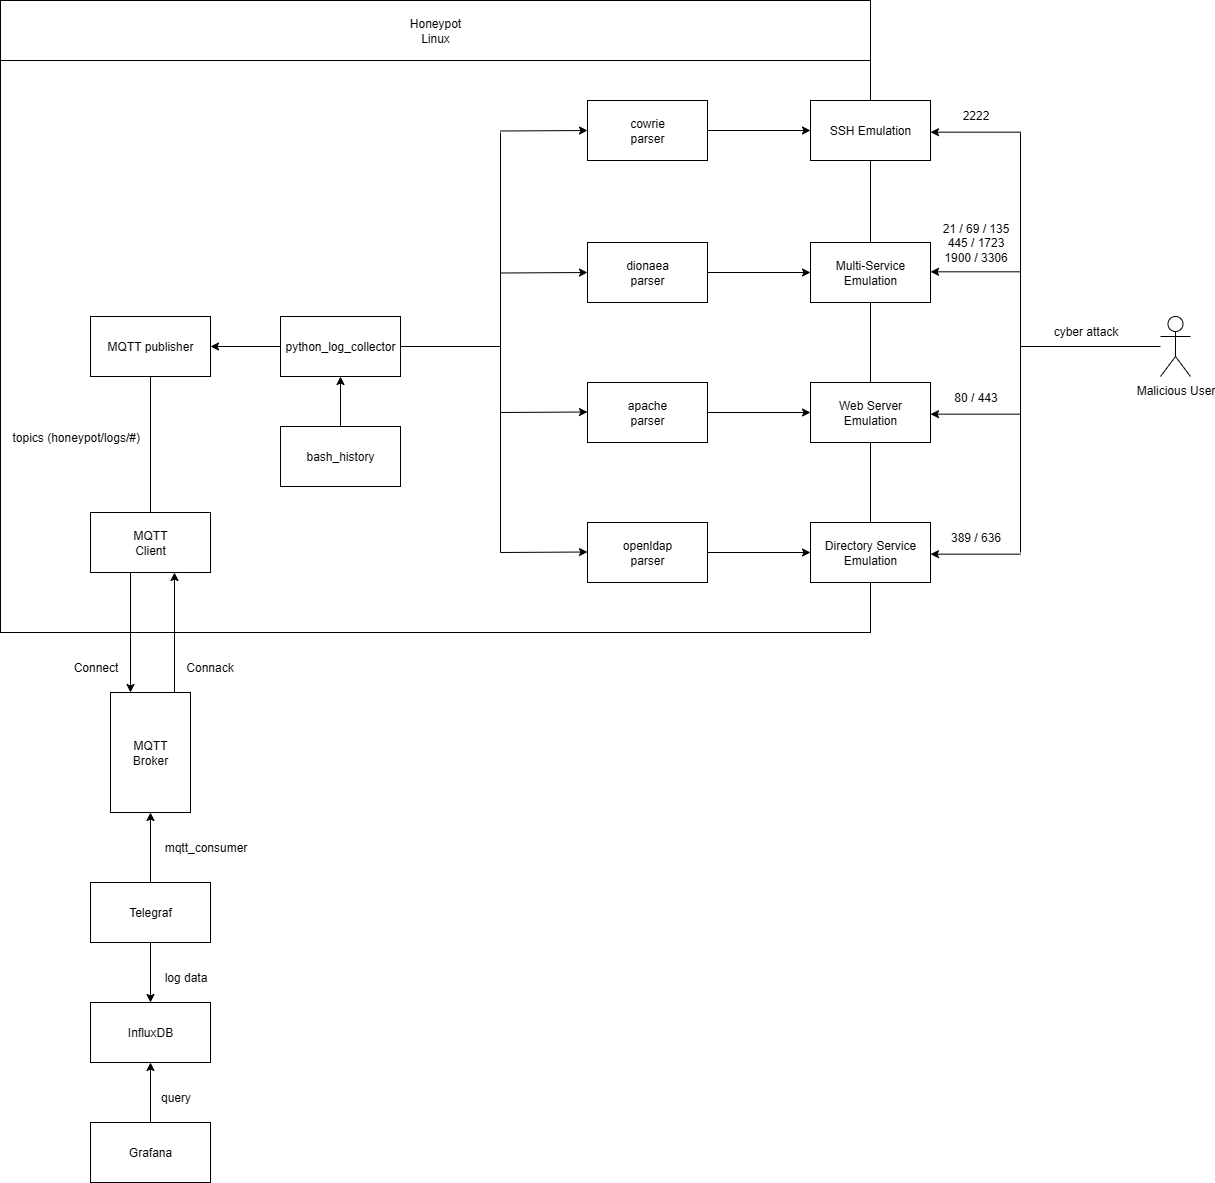
\includegraphics[width=1.025\textwidth]{img/Diagramma-flusso.png}
    \caption{Diagramma di flusso del sistema \textit{honeypot}.}
    \label{fig:flowchart}
    \end{center}
\end{figure}
Il diagramma mostra come i \textit{log} vengano generati dai servizi vulnerabili in seguito a tentativi di accesso o attacchi.
Gli \textit{script} di monitoraggio raccolgono i \textit{log}, li elaborano e li pubblicano su un \textit{topic} tramite un \textit{publisher} del protocollo \textit{MQTT}.
\textit{Telegraf}, poi, preleva i dati dal \textit{topic} e li invia al database \textit{InfluxDB} per la memorizzazione.
Infine, \textit{Grafana} consente di visualizzare i dati memorizzati nel database tramite \textit{dashboard} personalizzate.
\subsection{Scelta dei servizi del sistema}
Il sistema \textit{honeypot} doveva risultare realisticamente vulnerabile, in modo da attirare l'attenzione di potenziali attaccanti e raccogliere dati utili per l'analisi delle minacce. 
Per questo motivo abbiamo selezionato servizi noti per le loro vulnerabilità e diffusione, in grado di coprire una varietà di protocolli e tecnologie. 
La scelta è ricaduta su \textit{Cowrie}, \textit{Dionaea}, \textit{Apache} e \textit{OpenLDAP}. Ho scelto e configurato ciascuno di questi servizi per scenari d'attacco specifici e per fornire dati di valore durante il processo di monitoraggio.\\\\
\textbf{Cowrie} è un servizio progettato per emulare un sistema \textit{Linux} accessibile tramite protocollo \gls{ssh}\glsadd{ssh_def}. La sua funzione principale è quella di raccogliere informazioni su tentativi di accesso non autorizzato e sulle attività post-compromissione degli attaccanti. 
Per questo motivo l'ho configurato per ascoltare sulla porta 2222, simulando un server \textit{SSH} con un ambiente Linux realistico. 
Cowrie offre un \textit{file system} virtuale, l'emulazione di numerosi comandi \textit{bash} e il \textit{logging} completo delle sessioni, registrando anche eventuali \textit{upload} o \textit{download} di file tramite \gls{scp}\glsadd{scp_def} o \textit{wget}. 
La sua capacità di simulare vulnerabilità comuni lo rende particolarmente adatto a intercettare interazioni malevole e a raccogliere indicatori di compromissione.\\\\
\textbf{Dionaea}, invece, l'abbiamo scelto per la sua capacità di emulare più servizi vulnerabili contemporaneamente e di catturare \textit{payload} malevoli. 
Questo lo rende particolarmente utile nell'osservare attacchi automatizzati mirati a protocolli obsoleti o insicuri. 
Il \textit{container} l'ho configurato per ascoltare su diverse porte critiche: la 21 (\textit{FTP}), la 69 (\gls{tftp}), la 445 (\textit{SMB}), la 135 (\gls{rpc})\glsadd{rpc_def}, la 1723 (\gls{pptp}\glsadd{pptp_def}) e la 3306 (\textit{MySQL}). 
In questo modo \textit{Dionaea} è in grado di registrare tentativi di \textit{brute-force}, trasferimenti di file sospetti, comandi \gls{sql}\glsadd{sql_def} malevoli e attacchi legati a vulnerabilità precedentemente sfruttate. 
La sua versatilità consente di coprire un ampio spettro di minacce legate a servizi di rete differenti.\\\\
\textbf{Apache} lo abbiamo incluso per la sua enorme diffusione come server \textit{web} e per la frequente presenza di vulnerabilità legate al mondo delle applicazioni \textit{web}. 
Configurato per rispondere sulle porte 80 (\gls{http}\glsadd{http_def}) e 443 (\gls{https}\glsadd{https_def}), può essere utilizzato per simulare scenari di attacco tipici del \textit{web}, come \textit{directory traversal}, \textit{upload} di file non autorizzati, \gls{xss}\glsadd{xss_def} o altre iniezioni lato server. 
In tal modo è possibile raccogliere dati relativi a una delle superfici di attacco più comuni e sfruttate dagli attori malevoli.\\\\
Infine, l'ho integrato \textbf{OpenLDAP}, scelto per simulare un servizio di directory largamente utilizzato in ambito aziendale per l'autenticazione e la gestione centralizzata degli utenti. 
Il \textit{container} l'ho configurato per esporre sia la porta 389 (\gls{ldap} in chiaro) sia la 636 (\gls{ldaps} cifrato). 
Questa configurazione consente di osservare tentativi di enumerazione utenti, iniezione \textit{LDAP} e altre tecniche di compromissione legate a \textit{directory service}, che rappresentano spesso un obiettivo strategico per gli attaccanti al fine di ottenere accessi privilegiati.
La combinazione di questi servizi consente al sistema di coprire una grande varietà di scenari d'attacco: dall'accesso remoto tramite \textit{SSH}, alle compromissioni multi-protocollo, fino agli attacchi \textit{web} e ai tentativi di abuso di \textit{directory service}. 
In questo modo l'\textit{honeypot} risulta non solo realistico, ma anche utile per raccogliere dati diversificati e rappresentativi delle principali minacce informatiche attuali.
\subsection*{Diagramma delle classi e design pattern}
In seguito ho sviluppato il diagramma delle classi \textit{UML}, che rappresenta le principali classi e le loro relazioni all'interno del sistema.
\begin{figure}[H]
    \begin{center}
    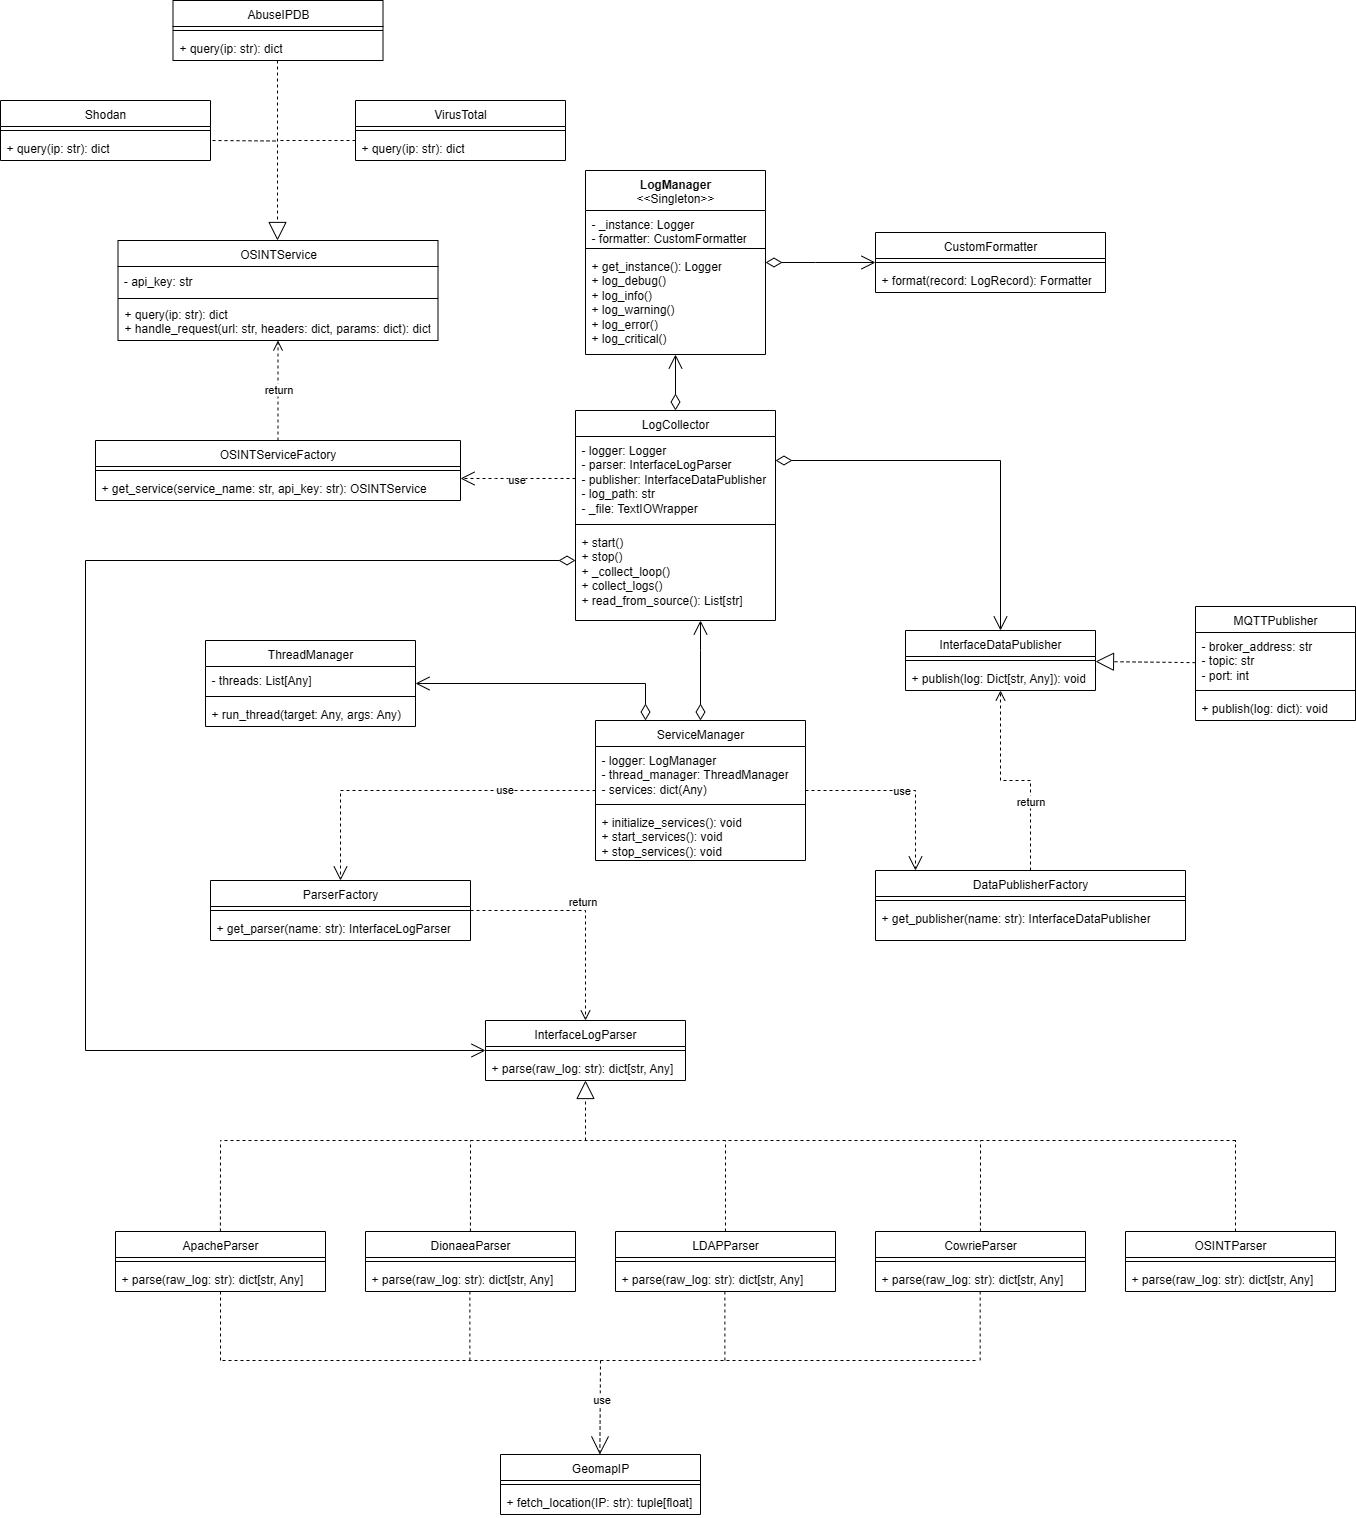
\includegraphics[width=\textwidth]{img/Diagramma-classi.png}
    \caption{Diagramma delle classi del sistema \textit{honeypot}.}
    \label{fig:class-diagram}
    \end{center}
\end{figure}
Per la progettazione del sistema e la realizzazione del relativo diagramma ho applicato diversi \textit{design pattern} studiati durante il corso di Ingegneria del \textit{Software}. 
Un primo esempio è rappresentato dal \textbf{\textit{Factory pattern}}, utilizzato nella classe \textit{ParserFactory}, la quale ha il compito di istanziare i diversi oggetti \textit{parser} a seconda del servizio vulnerabile da analizzare. 
In questo modo la logica di creazione viene centralizzata e resa indipendente dal resto del sistema, favorendo estendibilità e manutenibilità. 
Un ulteriore contributo deriva dall'applicazione dell'\textbf{\textit{Adapter pattern}}, che ha permesso di uniformare i \textit{log} provenienti da sorgenti differenti adattandoli al formato richiesto dal \textit{publisher} MQTT; tale approccio consente di integrare componenti con interfacce distinte senza doverne modificare l'implementazione originaria. 
La gestione centralizzata dei \textit{log} è invece garantita dal \textbf{\textit{Singleton pattern}}, applicato alla classe \textit{LogManager}, che deve esistere in un'unica istanza per tutta la durata dell'esecuzione del programma, evitando così conflitti dovuti alla creazione di istanze multiple. 
Per quanto riguarda le operazioni di \textit{parsing}, ho applicato lo \textbf{\textit{Strategy pattern}}, grazie al quale è possibile definire e incapsulare diverse strategie, una per ciascun servizio vulnerabile, e selezionare dinamicamente quella più appropriata durante l'esecuzione. 
L'\textbf{\textit{Observer pattern}} risulta applicato in maniera implicita attraverso l'uso del protocollo \textit{MQTT}: i moduli di monitoraggio pubblicano i \textit{log} su specifici \textit{topic}, ai quali \textit{Telegraf} si iscrive per ricevere in tempo reale gli aggiornamenti. 
Questo meccanismo riflette il principio dell'\textit{Observer}, in cui i cambiamenti nello stato di un soggetto sono propagati automaticamente a tutti gli osservatori registrati.\\\\
Infine, la seguente tabella riassume le versioni realizzate, gli elementi modellati e il tempo dedicato alle attività di modellazione e configurazione del sistema:
\begin{center}
\begin{longtable}{|p{0.25\textwidth}|p{0.10\textwidth}|p{0.25\textwidth}|p{0.05\textwidth}|}
\hline
\multicolumn{1}{|c|}{\textbf{Artefatto}} & 
\multicolumn{1}{c|}{\textbf{Versioni create}} & 
\multicolumn{1}{c|}{\textbf{Elementi modellati}} & 
\multicolumn{1}{c|}{\textbf{Ore dedicate}} \\ 
\hline
\endfirsthead

\multicolumn{4}{c}{{\bfseries \tablename\ \thetable{} -- Continuo della tabella}}\\
\hline
\multicolumn{4}{|c|}{\textbf{Attività di modellazione e configurazione}} \\ \hline
\endhead

\hline \multicolumn{4}{|r|}{{Continua nella prossima pagina...}} \\ \hline
\endfoot

\endlastfoot

Diagramma di flusso sistema & 3 & 8 componenti principali & 12 \\ \hline
Diagramma delle classi UML & 4 & 21 classi, 5 design pattern & 28 \\ \hline
Configurazione servizi honeypot & 4 per servizio & 4 servizi (Cowrie, Dionaea, Apache, LDAP) & 40 \\ \hline

\caption{Tabella quantitativa delle attività di modellazione e configurazione.}
\label{tab:modellazione-configurazione}
\end{longtable}
\end{center}
\section{Codifica}
\subsection{Struttura del progetto}
\normalsize
La struttura del progetto è organizzata in diverse cartelle principali, ciascuna con una responsabilità specifica. La cartella \texttt{config} contiene i \textit{file} per la configurazione dell'applicazione, includendo \texttt{environment\_config.py} per la gestione delle variabili e dei parametri di ambiente e \texttt{\_\_init\_\_.py} per l'inizializzazione della cartella stessa.\\
All'interno della cartella \texttt{core} si trovano i moduli fondamentali per l'esecuzione del sistema. \texttt{main.py} rappresenta l'\textit{entry point} dell'applicazione, mentre \texttt{geomap\_ip.py} si occupa della geolocalizzazione degli indirizzi IP. La raccolta dei \textit{log} viene gestita tramite \texttt{log\_collector.py}, la coordinazione dei servizi è affidata a \texttt{service\_manager.py} e l'esecuzione concorrente tramite \textit{thread} è curata da \texttt{thread\_manager.py}.\\
La cartella \texttt{logger} si dedica alla gestione centralizzata dei \textit{log}. \texttt{log\_manager.py} configura e gestisce il \textit{logger} principale, mentre \texttt{custom\_formatter.py} definisce formati personalizzati, ad esempio con codifica colore in base al livello di gravità.\\
Per quanto riguarda l'intelligence \textit{open source}, la cartella \texttt{osint} include moduli specifici. \texttt{base\_osint.py} definisce l'interfaccia comune per le integrazioni \textit{OSINT}, \texttt{osint\_factory.py} permette di istanziare dinamicamente i moduli come \texttt{abuseipdb.py}, \texttt{shodan.py} e \texttt{virustotal.py}, ciascuno dedicato a una diversa fonte di dati.\\
La cartella \texttt{parsers} raccoglie i parser per l'analisi e la normalizzazione dei \textit{log}. La classe base \texttt{base\_parser.py} definisce l'interfaccia comune, mentre \texttt{parser\_factory.py} consente di creare i \textit{parser} specifici per \texttt{cowrie\_parser.py}, \texttt{dionaea\_parser.py}, \texttt{apache\_parser.py}, \texttt{osint\_parser.py} e \texttt{LDAP\_parser.py}.\\
Infine, la cartella \texttt{publishers} contiene i moduli responsabili della pubblicazione dei \textit{log} verso sistemi esterni. \texttt{base\_publisher.py} definisce l'interfaccia astratta, \texttt{mqtt\_publisher.py} implementa un \textit{publisher} basato su \textit{MQTT} e \texttt{publisher\_factory.py} permette di creare dinamicamente i \textit{publisher} in base al contesto operativo.\\
Per rappresentare visivamente questa struttura, è possibile utilizzare il seguente albero:\\

\dirtree{%
.1 src/.
.2 config/.
.3 \_\_init\_\_.py.
.3 environment\_config.py.
.2 core/.
.3 \_\_init\_\_.py.
.3 main.py.
.3 geomap\_ip.py.
.3 log\_collector.py.
.3 service\_manager.py.
.3 thread\_manager.py.
.2 logger/.
.3 \_\_init\_\_.py.
.3 custom\_formatter.py.
.3 log\_manager.py.
.2 osint/.
.3 \_\_init\_\_.py.
.3 base\_osint.py.
.3 abuseipdb.py.
.3 shodan.py.
.3 virustotal.py.
.3 osint\_factory.py.
.2 parsers/.
.3 \_\_init\_\_.py.
.3 base\_parser.py.
.3 parser\_factory.py.
.3 cowrie\_parser.py.
.3 dionaea\_parser.py.
.3 apache\_parser.py.
.3 osint\_parser.py.
.3 LDAP\_parser.py.
.2 publishers/.
.3 \_\_init\_\_.py.
.3 base\_publisher.py.
.3 mqtt\_publisher.py.
.3 publisher\_factory.py.
}
In conclusione, le tabelle seguenti sintetizzano la dimensione e la complessità delle componenti sviluppate, riportando linee di codice, file creati e funzioni/metodi implementati. Esse illustrano inoltre le configurazioni e gli \textit{script} ausiliari realizzati per l'implementazione e l'automazione dei servizi, specificando quantità e descrizione di ciascun tipo di file.
\begin{center}
\begin{longtable}{|p{0.25\textwidth}|p{0.15\textwidth}|p{0.15\textwidth}|p{0.2\textwidth}|}
\hline
\multicolumn{1}{|c|}{\textbf{Componente}} & 
\multicolumn{1}{c|}{\textbf{Linee di codice}} & 
\multicolumn{1}{c|}{\textbf{File creati}} & 
\multicolumn{1}{c|}{\textbf{Funzioni/Metodi}} \\ 
\hline
\endfirsthead

\multicolumn{4}{c}{{\bfseries \tablename\ \thetable{} -- Continuo della tabella}}\\
\hline
\multicolumn{4}{|c|}{\textbf{Metriche di implementazione}} \\ \hline
\endhead

\hline \multicolumn{4}{|r|}{{Continua nella prossima pagina...}} \\ \hline
\endfoot

\endlastfoot

\textit{Core system} & 305 & 5 & 15 \\ \hline
\textit{Logger module} & 79 & 2 & 4 \\ \hline
\textit{Parsers} & 404 & 7 & 7 \\ \hline
\textit{Publishers} & 80 & 3 & 18 \\ \hline
\textit{OSINT integrations} & 108 & 5 & 7 \\ \hline
\textit{Configuration} & 32 & 1 & 1 \\ \hline
\textbf{TOTALE} & \textbf{1.008} & \textbf{23} & \textbf{52} \\ \hline

\caption{Tabella quantitativa delle metriche di implementazione del codice.}
\label{tab:metriche-codice}
\end{longtable}
\end{center}

\begin{center}
\begin{longtable}{|p{0.25\textwidth}|p{0.1\textwidth}|p{0.15\textwidth}|p{0.3\textwidth}|}
\hline
\multicolumn{1}{|c|}{\textbf{Tipo}} & 
\multicolumn{1}{c|}{\textbf{Quantità}} & 
\multicolumn{1}{|c|}{\textbf{Numero di versioni}} & 
\multicolumn{1}{c|}{\textbf{Descrizione}} \\ 
\hline
\endfirsthead

\multicolumn{3}{c}{{\bfseries \tablename\ \thetable{} -- Continuo della tabella}}\\
\hline
\multicolumn{3}{|c|}{\textbf{Configurazioni e \textit{script} ausiliari}} \\ \hline
\endhead

\hline \multicolumn{3}{|r|}{{Continua nella prossima pagina...}} \\ \hline
\endfoot

\endlastfoot

\textit{Docker Compose files} & 2 & 5 & Orchestrazione dei servizi \\ \hline
\textit{Dockerfile} & 3 & 4 & \textit{Container} personalizzati \\ \hline
\textit{Script Bash} & 1 & 3 & Automazione del \textit{deployment} \\ \hline
\textit{File} di configurazione \textit{Grafana} & 2 & 10 & \textit{Dashboard} e pannelli \\ \hline
\textit{File} di configurazione \textit{Telegraf} & 1 & 5 & \textit{Pipeline} per la raccolta dati \\ \hline

\caption{Tabella quantitativa delle configurazioni e degli \textit{script} ausiliari.}
\label{tab:configurazioni-script}
\end{longtable}
\end{center}

\subsection{Difficoltà incontrate}
Durante lo sviluppo del progetto, uno dei principali ostacoli riscontrati è rappresentato dalla complessità nel rielaborare i \textit{log} generati dai diversi servizi. Questi dati, provenienti dall'\textit{honeypot} e da sistemi ausiliari, presentavano formati variabili, richiedendo l'implementazione di espressioni regolari altamente specifiche e flessibili. La difficoltà consisteva non solo nel catturare correttamente le informazioni rilevanti, ma anche nel garantire la robustezza dei \textit{parser} di fronte a formati imprevisti o a \textit{log} contenenti dati inconsistenti, senza interrompere il flusso complessivo di raccolta e analisi. Ho superato questo problema mediante l'utilizzo del \textit{logger} interno del sistema per tracciare gli errori di parsing tramite messaggi di \textit{debug}, permettendo di identificare e correggere rapidamente le espressioni regolari difettose.
Un secondo aspetto critico riguardava la gestione della \textit{containerizzazione} tramite \textit{Docker} delle diverse componenti del sistema. La necessità di isolare i moduli, garantire l'interoperabilità tra servizi e preservare la sicurezza dell'ambiente ha reso necessario progettare con attenzione la rete dei \textit{container}, i volumi per la persistenza dei dati e la configurazione delle dipendenze. Problemi di compatibilità tra immagini, errori nella definizione dei \textit{Dockerfile} e difficoltà nella sincronizzazione dei \textit{container} tra loro hanno inizialmente rallentato le fasi di \textit{test} e \textit{deployment}. Sono riuscito a superare queste difficoltà grazie a una pianificazione accurata della struttura dei \textit{container}, all'uso di immagini standardizzate e alla creazione di \textit{script} di avvio automatizzati, consentendo di ottenere un ambiente stabile, sicuro e facilmente riproducibile.\\\\

\section{Verifica}
\subsection{Test}
La sezione illustra il metodo seguito per condurre le attività di testing, descrivendo i diversi tipi di test implementati e gli strumenti utilizzati per garantire la qualità del software.
\section{Validazione}
La validazione rappresenta la fase conclusiva del processo di sviluppo, volta a garantire che il sistema \textit{software} realizzato risponda effettivamente alle esigenze e ai requisiti definiti in fase di analisi. A differenza della verifica, che si concentra sul corretto funzionamento del prodotto rispetto alle specifiche tecniche, la validazione ha come obiettivo principale quello di accertare la coerenza del sistema rispetto agli obiettivi aziendali e operativi prefissati.  

Per raggiungere tale scopo ho seguito una metodologia strutturata che ha previsto:
\begin{itemize}
    \item la definizione di scenari di attacco realistici, basati su casi d'uso e minacce tipiche;
    \item l'impiego di strumenti consolidati per la simulazione, come \textit{Nmap} per la scansione delle porte e \textit{Hydra} per attacchi di \textit{brute-force};
    \item l'esecuzione di \textit{test} pratici sui servizi vulnerabili dell'\textit{honeypot}, con particolare attenzione alla generazione, raccolta e visualizzazione dei \textit{log}.
\end{itemize}

Ho condotto le attività con un approccio incrementale: inizialmente ho testato ogni servizio singolarmente, per poi essere validarli nel contesto del sistema integrato. Questo mi ha permesso di verificare non solo la robustezza dei singoli moduli, ma anche la correttezza del flusso complessivo dei dati dal momento dell'attacco simulato fino alla loro visualizzazione nei sistemi di monitoraggio.  

Le fasi di validazione si sono svolte nell'arco di una settimana, l'ultima dello \textit{stage}, con revisioni e confronti quotidiani con il tutor aziendale, il quale ha seguito da vicino tutte le attività, fornendo indicazioni e approvazioni parziali. Al termine del processo, il tutor ha rilasciato la propria approvazione finale, confermando la validità del sistema sviluppato.  

\subsection*{Conformità ai requisiti}
\label{requisiti-soddisfatti}
Dei requisiti iniziali definiti nella sezione \hyperref[requisiti]{requisiti}, il sistema sviluppato soddisfa pienamente tutti i requisiti funzionali, non funzionali e di vincolo.
Sebbene i requisiti non vadano a coprire completamente tutte le funzionalità richieste dagli obiettivi del progetto, il sistema risulta comunque essere un prodotto valido e funzionante, in grado di monitorare e analizzare efficacemente i tentativi di attacco sui servizi vulnerabili selezionati.
\begin{center}
\begin{longtable}{|p{0.2\textwidth}|p{0.75\textwidth}|}
\hline
\multicolumn{1}{|c|}{\textbf{Categoria}} & \multicolumn{1}{c|}{\textbf{Percentuale soddisfatta}}\\ 
\hline 
\endfirsthead
\multicolumn{2}{c}{{\bfseries \tablename\ \thetable{} -- Continuo della tabella}}\\
\hline
\multicolumn{1}{|c|}{\textbf{Categoria}} & \multicolumn{1}{c|}{\textbf{Percentuale soddisfatta}}\\ \hline 
\endhead
\hline
\multicolumn{2}{|r|}{{Continua nella prossima pagina...}}\\
\hline
\endfoot
\endlastfoot 

Funzionali & 100\%\\ \hline
Non funzionali & 100\%\\ \hline
Vincolo & 100\%\\ \hline
\caption{Requisiti soddisfatti dal sistema sviluppato.}
\label{tab:requisiti-soddisfatti}
\end{longtable}
\end{center}

\subsection*{Risultati quantitativi}
Complessivamente, abbiamo eseguito oltre trenta scenari di simulazioni di attacco, comprendenti scansioni, \textit{brute-force} e caricamenti di file malevoli. Tutti e quattro i servizi vulnerabili previsti hanno ricevuto la validazione ottenendo quattro tipologie distinte di \textit{log}, a conferma della tracciabilità completa lungo la \textit{pipeline} di raccolta e visualizzazione.
Facendo ciò abbiamo raggiunto i seguenti dati di validazione:

\begin{center}
\begin{longtable}{|p{0.18\textwidth}|p{0.15\textwidth}|p{0.35\textwidth}|p{0.2\textwidth}|}
\hline
\multicolumn{1}{|c|}{\textbf{Servizio}} & 
\multicolumn{1}{c|}{\textbf{Scenari testati}} & 
\multicolumn{1}{c|}{\textbf{Tipologie attacchi}} & 
\multicolumn{1}{c|}{\textbf{\textit{Log} generati}} \\ 
\hline
\endfirsthead

\multicolumn{4}{c}{{\bfseries \tablename\ \thetable{} -- Continuo della tabella}}\\
\hline
\multicolumn{4}{|c|}{\textbf{Scenari di attacco testati}} \\ \hline
\endhead

\hline \multicolumn{4}{|r|}{{Continua nella prossima pagina...}} \\ \hline
\endfoot

\endlastfoot

\textit{Cowrie (SSH)} & 12 & \textit{Brute-force, command injection} & 86 eventi \\ \hline
\textit{Dionaea} & 8 & \textit{Multi-protocol, malware upload} & 77 eventi \\ \hline
\textit{Apache} & 7 & \textit{Directory traversal, XSS} & 34 eventi \\ \hline
\textit{OpenLDAP} & 6 & \textit{LDAP injection, enumeration} & 28 eventi \\ \hline
\textbf{TOTALE} & 33 & 8 tipologie & 225 eventi \\ \hline

\caption{Tabella quantitativa degli scenari di attacco testati e dei \textit{log} generati.}
\label{tab:scenari-attacco}
\end{longtable}
\end{center}


\begin{center}
\begin{longtable}{|p{0.15\textwidth}|p{0.15\textwidth}|p{0.25\textwidth}|p{0.3\textwidth}|}
\hline
\multicolumn{1}{|c|}{\textbf{Strumento}} & 
\multicolumn{1}{c|}{\textbf{Scansioni eseguite}} & 
\multicolumn{1}{c|}{\textbf{Parametri testati}} & 
\multicolumn{1}{c|}{\textbf{Risultati ottenuti}} \\ 
\hline
\endfirsthead

\multicolumn{4}{c}{{\bfseries \tablename\ \thetable{} -- Continuo della tabella}}\\
\hline
\multicolumn{4}{|c|}{\textbf{Strumenti e risultati di \textit{testing}}} \\ \hline
\endhead

\hline \multicolumn{4}{|r|}{{Continua nella prossima pagina...}} \\ \hline
\endfoot

\endlastfoot

\textit{Nmap} & 12 & Porte, servizi, \textit{OS detection} & 100\% servizi rilevati \\ \hline
\textit{Hydra} & 8 & \textit{Brute-force SSH, FTP} & 100\% tentativi \textit{loggati} \\ \hline
\textit{LDAP-utils} & 6 & \textit{LDAP queries, file upload} & 100\% eventi tracciati \\ \hline

\caption{Tabella quantitativa degli strumenti e dei risultati dei \textit{test}.}
\label{tab:strumenti-testing}
\end{longtable}
\end{center}

L'insieme di queste attività, unite all'approvazione del tutor aziendale, dimostra che il sistema soddisfa i requisiti funzionali, non funzionali e di vincolo definiti in fase di analisi, garantendo affidabilità, correttezza e coerenza operativa del prodotto sviluppato.

\section{Visione d'insieme}
In questa sezione sono presenti i risultati ottenuti durante lo sviluppo del progetto, confrontandoli con gli obiettivi iniziali e valutando il successo del progetto stesso.
\subsection{Prodotto finale}
Il prodotto finale del progetto è un sistema \textit{honeypot} modulare e scalabile, in grado di monitorare e analizzare tentativi di attacco su vari servizi di rete.
Nelle figure seguenti sono mostrate le principali componenti del sistema, che spaziano dalla configurazione iniziale del \textit{logger}, alla gestione del \textit{database} tramite \textit{InfluxDB}, fino alla visualizzazione dei dati attraverso le \textit{dashboard} interattive fornite da \textit{Grafana}.
\begin{figure}[H]
    \begin{center}
    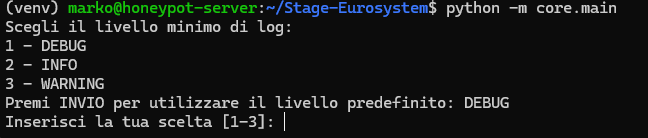
\includegraphics[width=\textwidth]{img/environment.png}
    \caption{Scelta del livello minimo del \textit{logger} al momento dell'inizializzazione.}
    \label{fig:environment}
    \end{center}
\end{figure}
\begin{figure}[H]
    \begin{center}
    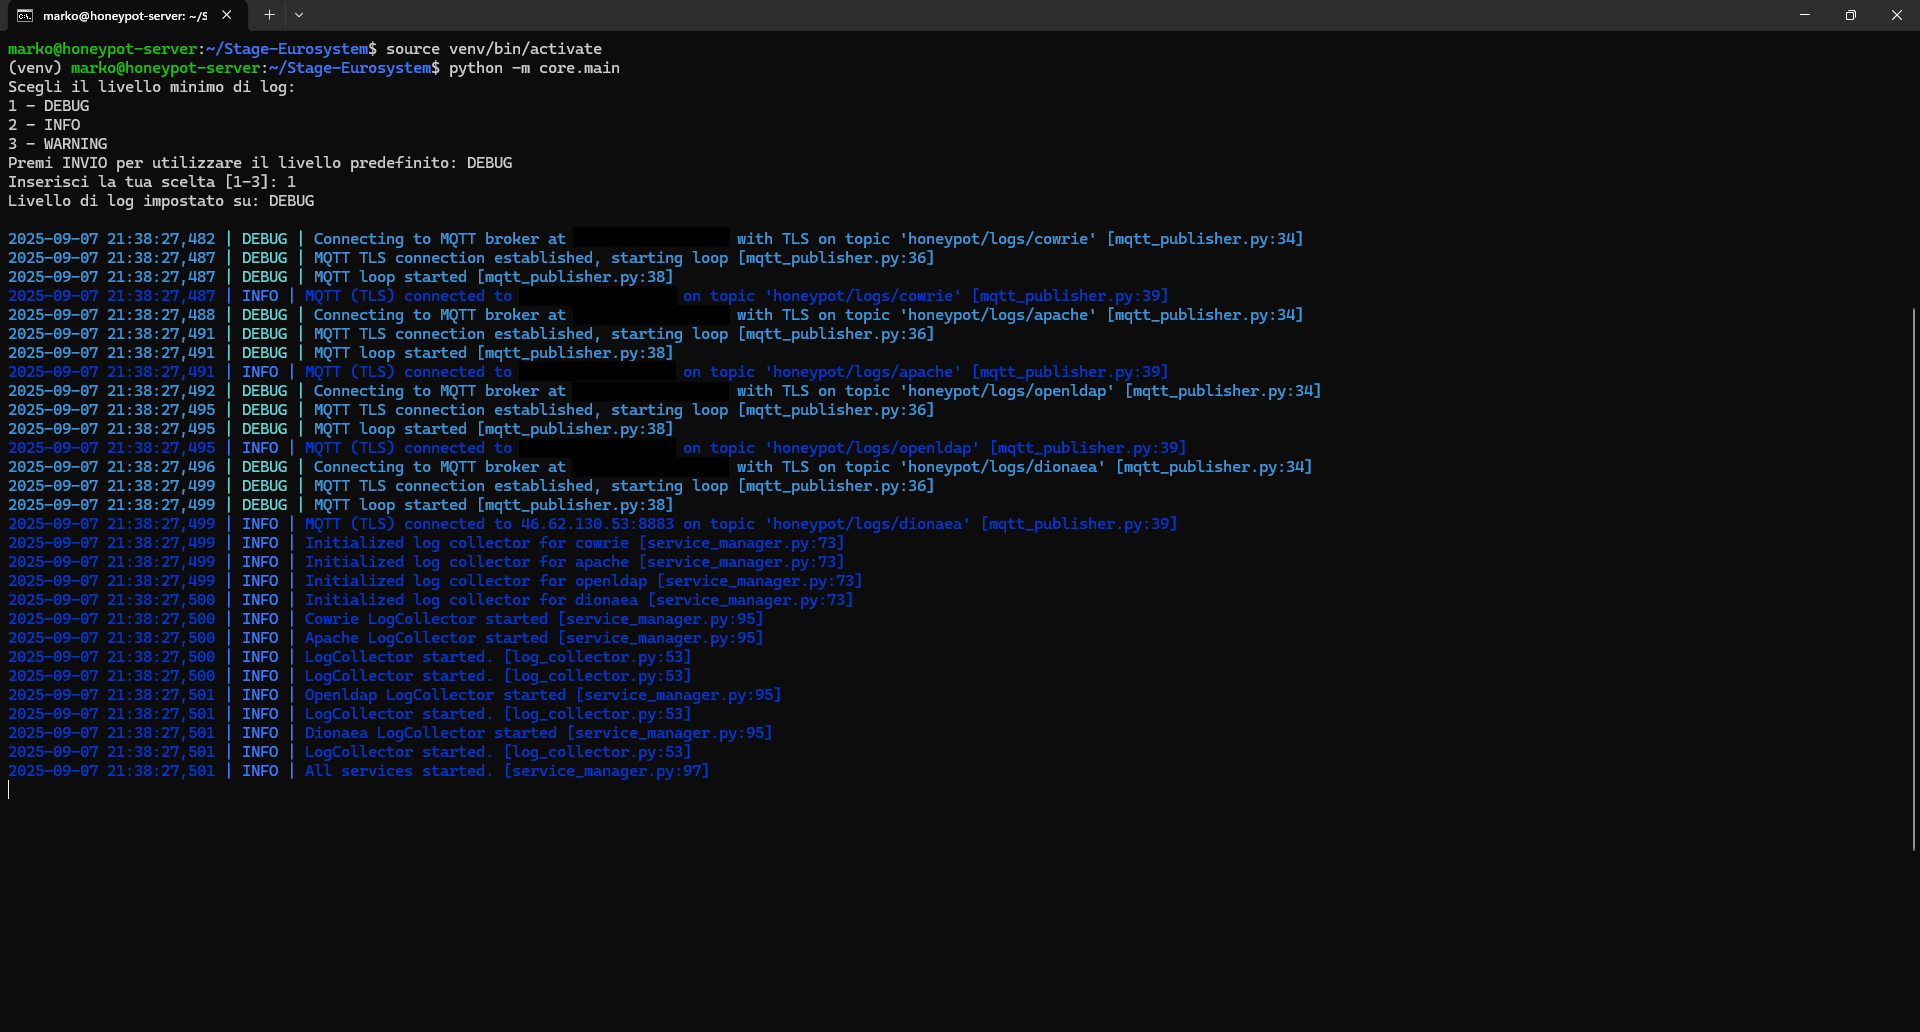
\includegraphics[width=\textwidth]{img/logger.png}
    \caption{Esempio di \textit{logger} in funzione in modalità \textit{debug}.}
    \label{fig:logger}
    \end{center}
\end{figure}
\begin{figure}[H]
    \begin{center}
    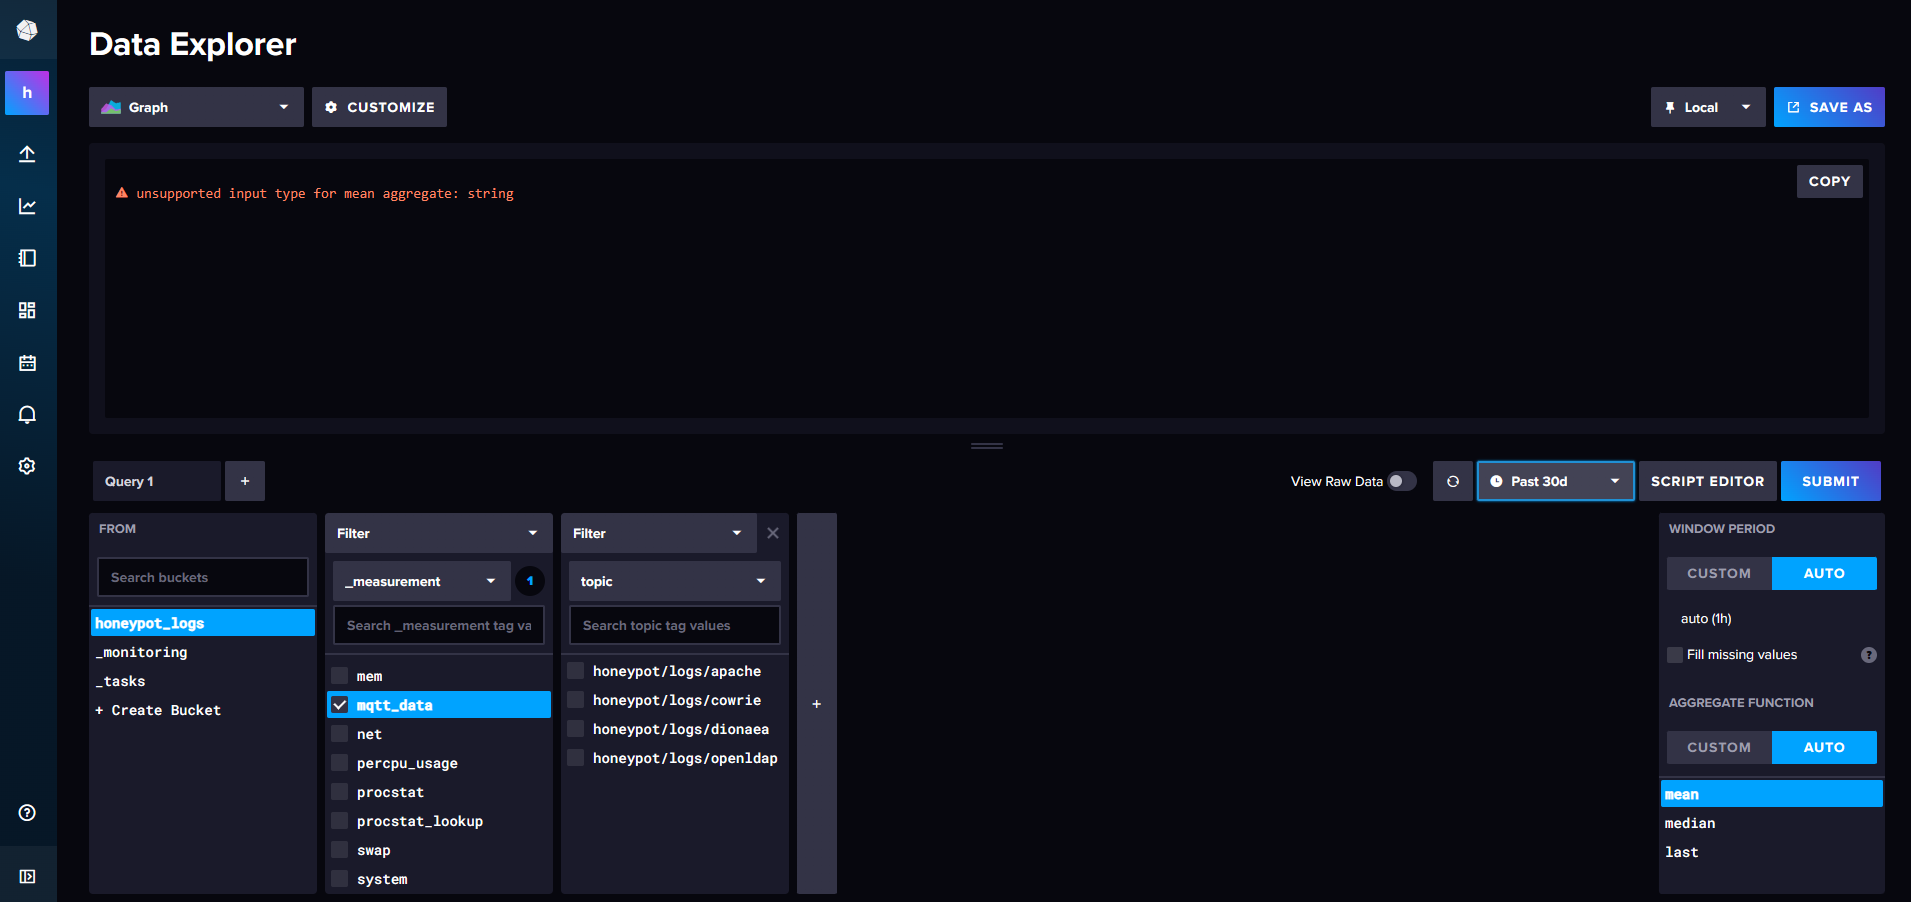
\includegraphics[width=\textwidth]{img/influxdb.png}
    \caption{Interfaccia web di \textit{InfluxDB} per la gestione del \textit{database}.}
    \label{fig:influxdb}
    \end{center}
\end{figure}
\begin{figure}[H]
    \begin{center}
    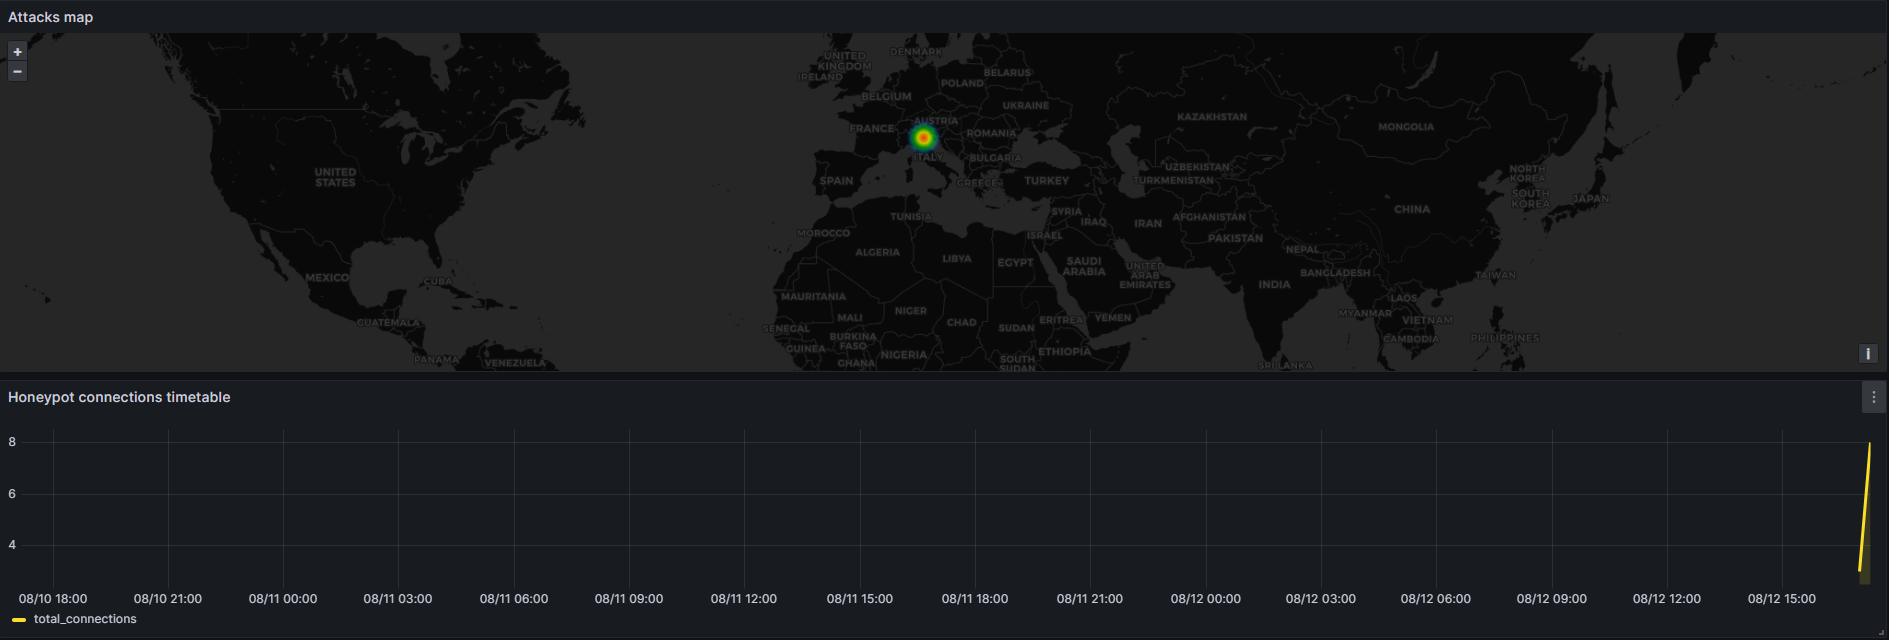
\includegraphics[width=\textwidth]{img/grafana-1.png}
    \caption{Esempio di \textit{dashboard} di \textit{Grafana} per la visualizzazione dei dati raccolti dall'\textit{honeypot}.}
    \label{fig:grafana-1}
    \end{center}
\end{figure}
\begin{figure}[H]
    \begin{center}
    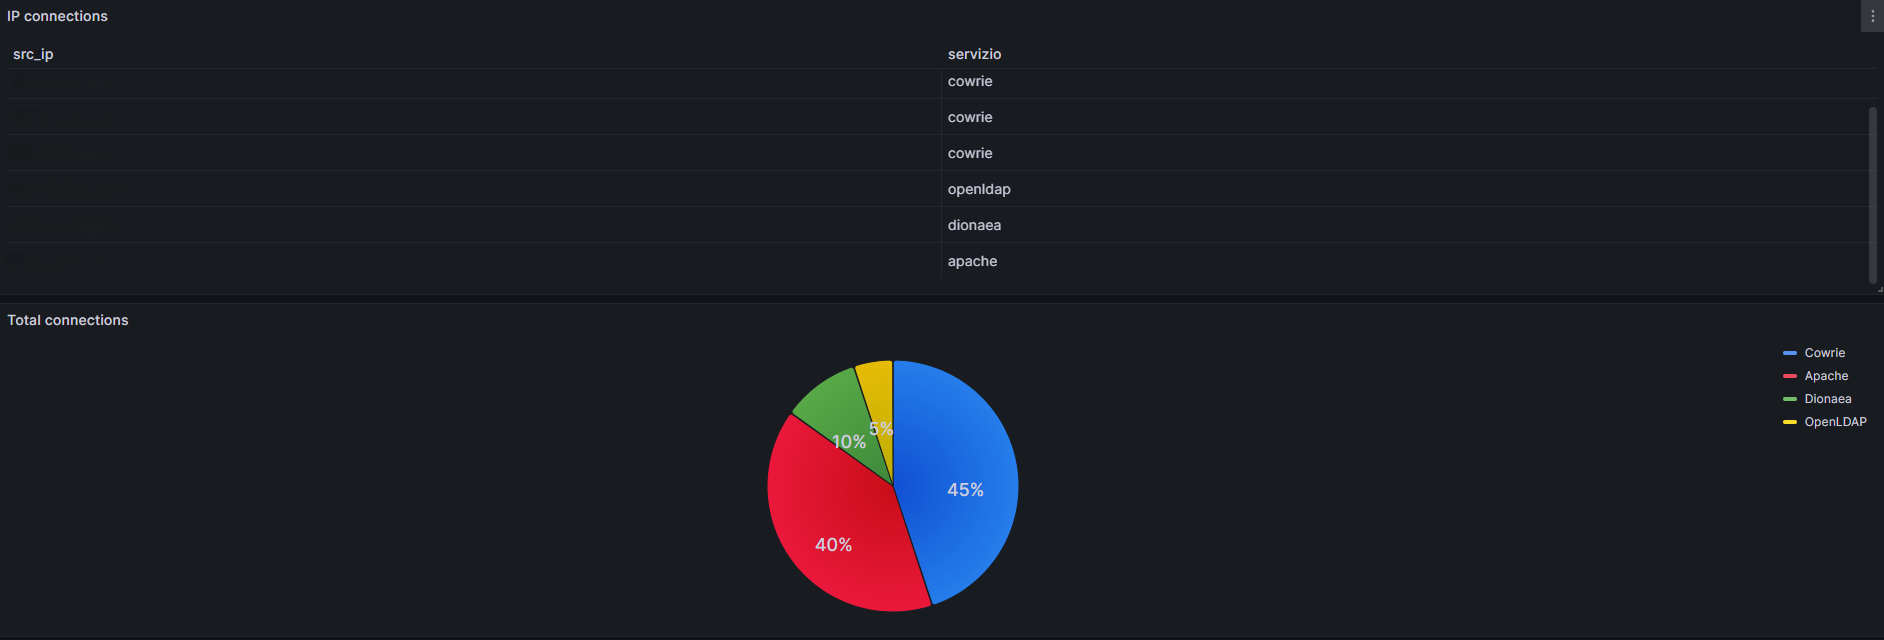
\includegraphics[width=\textwidth]{img/grafana-2.png}
    \caption{Esempio di \textit{dashboard} di \textit{Grafana} per la visualizzazione dei dati raccolti dall'\textit{honeypot}.}
    \label{fig:grafana-2}
    \end{center}
\end{figure}
\begin{figure}[H]
    \begin{center}
    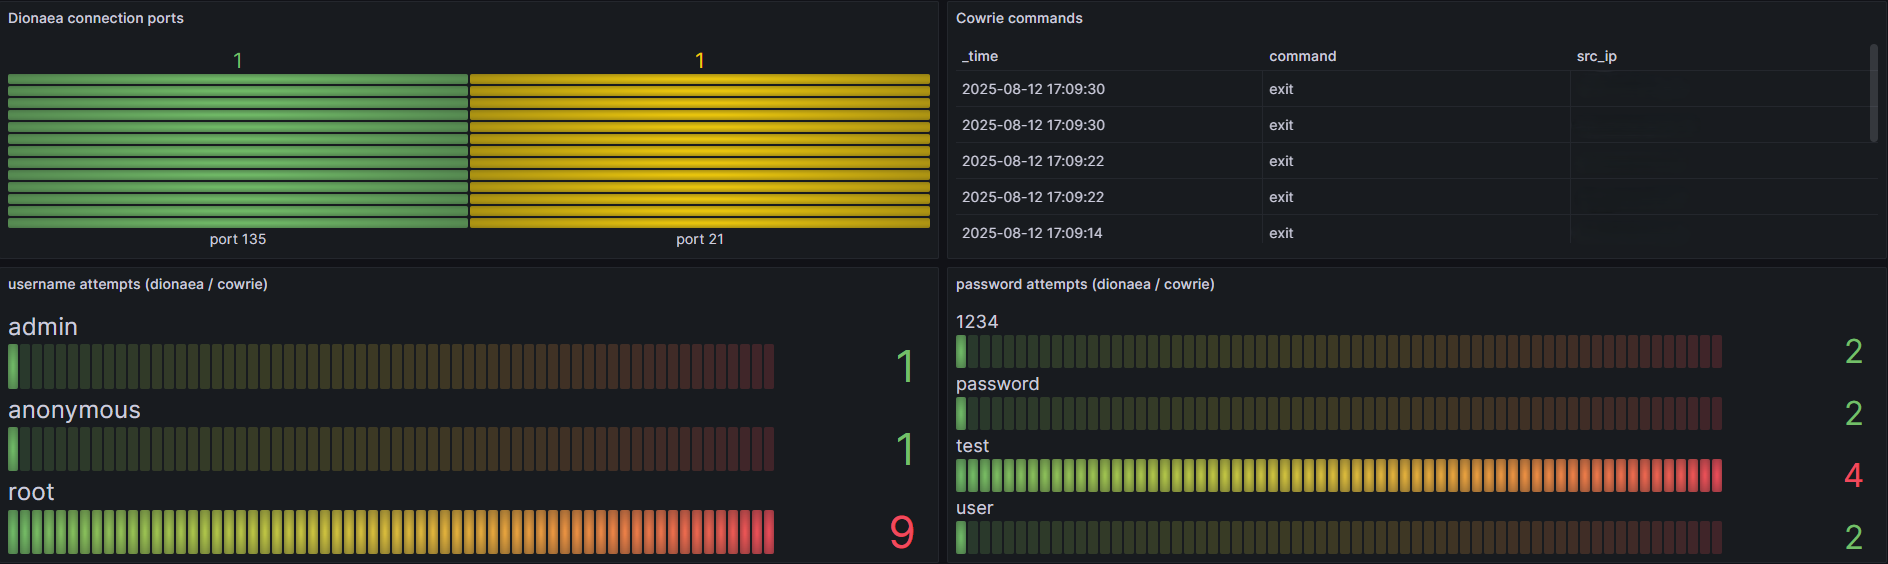
\includegraphics[width=\textwidth]{img/grafana-3.png}
    \caption{Esempio di \textit{dashboard} di \textit{Grafana} per la visualizzazione dei dati raccolti dall'\textit{honeypot}.}
    \label{fig:grafana-3}
    \end{center}
\end{figure}
Gli indirizzi \textit{IP} sono opportunamente mascherati per motivi di sicurezza.
    \chapter{Valutazione retrospettiva}
\label{cap:valutazione-retrospettiva}
Il quarto capitolo presenta un giudizio delle attività svolte durante lo \textit{stage}, ponendo particolare attenzione al confronto tra le competenze professionali maturate nel corso dell'esperienza e quelle già possedute in precedenza.
\section{Obiettivi raggiunti}
La sezione ha l'obiettivo di fornire una valutazione dettagliata dei risultati ottenuti durante lo \textit{stage}, evidenziando quali e quanti degli obiettivi precedentemente definiti siano stati effettivamente raggiunti.
\section{Conoscenze acquisite}
Questa sezione elenca e descrive le nuove conoscenze acquisite durante lo stage, particolare riferimento alle tecnologie, metodologie e tecniche nel campo della cybersecurity e dello sviluppo \textit{software}.
\section{Competenze professionali acquisite}
In questa sezione si descrivono le competenze pratiche e professionali sviluppate durante l'esperienza di \textit{stage}, incluse competenze tecniche specifiche, capacità di \textit{problem solving} e abilità di lavoro in \textit{team} in ambiente professionale.

    \pagenumbering{roman}
    \backmatter
    \chapter{Bibliografia}
\label{cap:bibliography}

\nocite{*}

% Books bibliography
\printbibliography[heading=subbibliography, title={Testi}, type=book]

% Articles bibliography
\printbibliography[heading=subbibliography, title={Articoli}, type=article]

% Websites bibliography
%\printbibliography[heading=subbibliography, title={Siti}, type=online]

    \chapter{Sitografia}
\label{cap:webliography}
\nocite{*}

% Websites bibliography
\printbibliography[heading=subbibliography, title={\null}, type=online]

    \printglossary[type=\acronymtype, title=Acronimi e abbreviazioni, toctitle=Acronimi e abbreviazioni]
    \label{acronimi}
    \printglossary[type=main, title=Glossario, toctitle=Glossario]
    \label{glossario}
\end{document}